%Version 3.1 December 2024
% See section 11 of the User Manual for version history
%
%%%%%%%%%%%%%%%%%%%%%%%%%%%%%%%%%%%%%%%%%%%%%%%%%%%%%%%%%%%%%%%%%%%%%%
%%                                                                 %%
%% Please do not use \input{...} to include other tex files.       %%
%% Submit your LaTeX manuscript as one .tex document.              %%
%%                                                                 %%
%% All additional figures and files should be attached             %%
%% separately and not embedded in the \TeX\ document itself.       %%
%%                                                                 %%
%%%%%%%%%%%%%%%%%%%%%%%%%%%%%%%%%%%%%%%%%%%%%%%%%%%%%%%%%%%%%%%%%%%%%

%%\documentclass[referee,sn-basic]{sn-jnl}% referee option is meant for double line spacing

%%=======================================================%%
%% to print line numbers in the margin use lineno option %%
%%=======================================================%%

%%\documentclass[lineno,pdflatex,sn-basic]{sn-jnl}% Basic Springer Nature Reference Style/Chemistry Reference Style

%%=========================================================================================%%
%% the documentclass is set to pdflatex as default. You can delete it if not appropriate.  %%
%%=========================================================================================%%

%%\documentclass[sn-basic]{sn-jnl}% Basic Springer Nature Reference Style/Chemistry Reference Style

%%Note: the following reference styles support Namedate and Numbered referencing. By default the style follows the most common style. To switch between the options you can add or remove “Numbered in the optional parenthesis. 
%%The option is available for: sn-basic.bst, sn-chicago.bst%  
 
%%\documentclass[pdflatex,sn-nature]{sn-jnl}% Style for submissions to Nature Portfolio journals
%%\documentclass[pdflatex,sn-basic]{sn-jnl}% Basic Springer Nature Reference Style/Chemistry Reference Style
\documentclass[lineno,pdflatex,sn-mathphys-num]{sn-jnl}% Math and Physical Sciences Numbered Reference Style
%%\documentclass[pdflatex,sn-mathphys-ay]{sn-jnl}% Math and Physical Sciences Author Year Reference Style
%%\documentclass[pdflatex,sn-aps]{sn-jnl}% American Physical Society (APS) Reference Style
%%\documentclass[pdflatex,sn-vancouver-num]{sn-jnl}% Vancouver Numbered Reference Style
%%\documentclass[pdflatex,sn-vancouver-ay]{sn-jnl}% Vancouver Author Year Reference Style
%%\documentclass[pdflatex,sn-apa]{sn-jnl}% APA Reference Style
%%\documentclass[pdflatex,sn-chicago]{sn-jnl}% Chicago-based Humanities Reference Style

%%%% Standard Packages
%%<additional latex packages if required can be included here>

\usepackage{graphicx}%
\usepackage{multirow}%
\usepackage{amsmath,amssymb,amsfonts}%
\usepackage{amsthm}%
\usepackage{mathrsfs}%
\usepackage[title]{appendix}%
\usepackage{xcolor}%
\usepackage{textcomp}%
\usepackage{manyfoot}%
\usepackage{booktabs}%
\usepackage{algorithm}%
\usepackage{algorithmicx}%
\usepackage{algpseudocode}%
\usepackage{listings}%
\usepackage{xurl}
\usepackage{placeins}
%%%%

%%%%%=============================================================================%%%%
%%%%  Remarks: This template is provided to aid authors with the preparation
%%%%  of original research articles intended for submission to journals published 
%%%%  by Springer Nature. The guidance has been prepared in partnership with 
%%%%  production teams to conform to Springer Nature technical requirements. 
%%%%  Editorial and presentation requirements differ among journal portfolios and 
%%%%  research disciplines. You may find sections in this template are irrelevant 
%%%%  to your work and are empowered to omit any such section if allowed by the 
%%%%  journal you intend to submit to. The submission guidelines and policies 
%%%%  of the journal take precedence. A detailed User Manual is available in the 
%%%%  template package for technical guidance.
%%%%%=============================================================================%%%%

%% as per the requirement new theorem styles can be included as shown below
\theoremstyle{thmstyleone}%
\newtheorem{theorem}{Theorem}%  meant for continuous numbers
%%\newtheorem{theorem}{Theorem}[section]% meant for sectionwise numbers
%% optional argument [theorem] produces theorem numbering sequence instead of independent numbers for Proposition
\newtheorem{proposition}[theorem]{Proposition}% 
%%\newtheorem{proposition}{Proposition}% to get separate numbers for theorem and proposition etc.

\theoremstyle{thmstyletwo}%
\newtheorem{example}{Example}%
\newtheorem{remark}{Remark}%

\theoremstyle{thmstylethree}%
\newtheorem{definition}{Definition}%

\raggedbottom
%%\unnumbered% uncomment this for unnumbered level heads

% \usepackage{amsmath}    % for \text{} inside equations
% \usepackage{multirow}   % optional, for merged table cells
% \usepackage{tikz}
% \usepackage{url}
% \usetikzlibrary{arrows.meta,positioning}
% \usetikzlibrary{calc}
% \usetikzlibrary{patterns}
% \usepackage{pgfplots}   % bar charts


\begin{document}

\title[Article Title]{Where Do Vision Foundation Models Look? A Comparative Study of Attention Alignment in Architectural Image Recognition}

%%=============================================================%%
%% GivenName	-> \fnm{Joergen W.}
%% Particle	-> \spfx{van der} -> surname prefix
%% FamilyName	-> \sur{Ploeg}
%% Suffix	-> \sfx{IV}
%% \author*[1,2]{\fnm{Joergen W.} \spfx{van der} \sur{Ploeg} 
%%  \sfx{IV}}\email{iauthor@gmail.com}
%%=============================================================%%

\author[1]{\fnm{Desmond} \sur{Choy}}\email{e1510259@u.nus.edu}
\author[1]{\fnm{Kay Mei} \sur{Leong}}\email{e0324286@u.nus.edu}
\author*[1]{\fnm{Jing} \sur{Tian}}\email{tianjing@nus.edu.sg}
\author[1]{\fnm{Xavier Zhen} \sur{Xie}}\email{xav.xie@nus.edu.sg}

\affil*[1]{\orgdiv{NUS-ISS}, \orgname{National University of Singapore}, \orgaddress{\street{25 Heng Mui Keng Terrace}, \city{Singapore}, \postcode{119615}, \country{Singapore}}}


%%==================================%%
%% Sample for unstructured abstract %%
%%==================================%%

\abstract{Vision foundation models achieve strong recognition performance, but it remains unclear whether their attention aligns with the visual evidence that human experts consider discriminative. This paper presents a comparative study of attention alignment in image recognition, using the WikiChurches benchmark dataset, in which expert-annotated bounding boxes identify style-relevant architectural features. The study examines the attention alignment by formulating three research questions: whether frozen models exhibit expert-aligned attention, how attention alignment varies across intermediate layers and heads, and how downstream adaptation changes attention alignment. This paper presents a comprehensive comparison of six vision foundation models, spanning image-only self-supervised and vision-language models, and measures attention alignment using five complementary metrics, three types of attention maps, and three adaptation strategies. The findings show that attention alignment provides a useful diagnostic lens beyond classification accuracy, while remaining evidence of spatial plausibility rather than causal explanation.}


\keywords{Explainable computer vision; vision foundation model; attention map; attentional alignment; image recognition}

%%\pacs[JEL Classification]{D8, H51}

%%\pacs[MSC Classification]{35A01, 65L10, 65L12, 65L20, 65L70}

\maketitle

%\clearpage

\section{Introduction}

Vision foundation models are trained on large-scale and diverse visual data, enabling them to serve as general-purpose representation backbones that can be adapted to a wide range of downstream tasks~\cite{Awais25PAMI}. As these models are increasingly deployed in critical applications, including medical image analysis and autonomous driving, understanding their decision-making behavior has become essential for interpretability and trustworthiness~\cite{Hasic26NN, Remi25IF, Wan26PAMI, Kashefi2026review}.

A central challenge is to reveal not only whether a vision foundation model predicts correctly, but also what visual evidence it uses to support its prediction. Existing visual explanation methods provide important tools for this purpose by highlighting image regions that contribute to model decisions. Representative methods include \textit{Gradient-weighted Class Activation Mapping} (Grad-CAM)~\cite{Selvaraju17GradCAM}, which localizes class-discriminative regions through gradient-based activation maps, and attention-based or relevance-propagation methods such as deep Taylor decomposition~\cite{Chefer21Interp}. These methods have improved the transparency of visual models by making their spatial evidence more accessible.

However, many existing explanation methods primarily focus on producing a final explanation for a model output. They provide limited insight into how discriminative attention emerges and evolves across the internal layers and attention heads of a model \cite{Voita19Heads}. This limitation is especially important for transformer-based vision foundation models, where intermediate blocks and heads may capture different visual patterns or object parts \cite{Caron21DINO}. Studying this internal evolution can help reveal how models progressively attend to diagnostically relevant regions, which layers or heads contribute most strongly to the final decision, and whether different components specialize in different types of visual evidence \cite{Raghu21ViTvsCNN}. Moreover, because pretrained vision foundation models are commonly adapted to downstream tasks, it is also important to examine how adaptation changes their attention behavior \cite{Kumar22Distort, Biderman24LoRA}. A model may improve its classification accuracy after fine-tuning, but this improvement does not necessarily imply better alignment with human-recognized evidence.

To address these questions, this paper presents a comparative study of attention alignment in vision foundation models for architectural image recognition. Architectural style recognition provides a particularly suitable setting because correct classification often depends on localized and semantically meaningful visual elements. The WikiChurches benchmark dataset~\cite{Barz21WikiChurches} offers a strong benchmark for this analysis because it provides fine-grained architectural-style labels together with expert-annotated bounding boxes that mark characteristic architectural elements. These annotations make it possible to evaluate model attention against human expert evidence rather than relying solely on class prediction accuracy.

This study is organized around three research questions. First, how well do frozen vision foundation models align their attention with expert-annotated architectural regions? Second, do intermediate layers and attention heads exhibit feature-specific specialization for different architectural elements? Third, how do different adaptation strategies, including linear probing, \textit{Low-Rank Adaptation} (LoRA) \cite{hu2022lora}, and full fine-tuning, affect attention alignment? By answering these questions, the study moves beyond final prediction accuracy performance and examines whether vision foundation models attend to visual evidence that is consistent with expert reasoning.

The contributions of this paper are threefold.
\begin{itemize}
\item First, we formulate attention alignment as an evaluation problem that measures the correspondence between attention maps from vision foundation models and expert-annotated architectural regions. This formulation enables systematic analysis of whether model attention is spatially consistent with human-recognized discriminative evidence.
\item Second, we study attention alignment along three complementary axes: model-level alignment, layer-level and head-level specialization, and adaptation-induced changes during downstream tuning. This design allows us to examine not only where models attend, but also how attention evolves internally and how it changes after task adaptation.
\item Third, we conduct a comprehensive empirical study covering six vision foundation models, three types of attention maps, three adaptation strategies, and five alignment metrics on a benchmark architectural image dataset. This provides a broad comparative view of how different pretraining paradigms and adaptation choices influence attention alignment.
\end{itemize}

The rest of this paper is organized as follows. Section~\ref{section related works} reviews prior work on explaining vision foundation models and evaluating model explanations, and highlights the distinction between this study and existing literature. Section~\ref{section proposed approach} presents the research questions and details the study design, including the evaluated models, attention maps, adaptation strategies, and performance metrics. Section~\ref{section results} reports the experimental results, analysis, and limitations. Finally, Section~\ref{section conclusions} concludes the paper.

\section{Related Work} \label{section related works}

\subsection{Explaining vision foundation models}

Many studies have shown how attention maps and activation-based visualizations can be used to explain the behavior of vision foundation models. These attention-based methods leverage the native self-attention structure of \textit{Vision Transformers} (ViTs) \cite{dosovitskiy21vit}. The raw attention visualization derived from the final transformer layers serves as a baseline inspection tool in the original ViT formulation. Furthermore, attention signals become progressively entangled across layers inside the ViT model \cite{Abnar20Rollout}.

For ViT interpretability, several methods refine the use of attention maps beyond simple averaging or raw visualization. Kang et al.~\cite{Kang20259339} investigate whether frozen large vision-language models contain attention heads that already encode object localization behavior. Rather than adding task-specific grounding heads or fine-tuning the model, their method identifies a small subset of localization heads. It uses text-to-image attention maps to recover image regions associated with textual descriptions. A gradient-driven multi-head attention rollout is proposed to estimate the relative importance of individual attention heads using gradient-derived scores, and then to aggregate head-level attention with learned weights \cite{Jo2025582}. This addresses the limitation that not all heads contribute equally to a model decision. A dynamic accumulated attention map is proposed to focus on the temporal evolution of attention across transformer blocks \cite{Liao2025PR}. By decomposing class-token representations and accumulating block-wise attention information, it emphasizes layer-wise attention flow and the formation of decision evidence inside the transformer.

Other works adapt attention-based explanations to weakly supervised or domain-specific prediction tasks. Hanna et al.~\cite{Hanna25ICCV} propose a sparse ViT with multiple class-specific \texttt{[CLS]} tokens for weakly supervised semantic segmentation. Their method encourages each class token to specialize through masking and then uses the corresponding self-attention maps to generate pseudo-segmentation masks. This differs from post-hoc explanation approaches because the model architecture and training procedure are designed to make class-specific attention more directly usable as an explanation. In medical imaging, Cascone et al.~\cite{Cascone25ICCV} build an interpretable diabetic retinopathy grading framework, using the transformer backbone as both a representation learner and a source of explanation for clinical decision support. Feng et al. \cite{Feng2025AI} propose counterfactual example generation for classifying wafer map failure patterns.


\subsection{Measuring model explanations}

The other related work evaluates what attention maps and visual explanations actually capture. The first category of works measures how training objectives influence internal attention mechanisms. Park et al.~\cite{park2023what} analyze self-supervised ViTs trained with contrastive learning and masked image modeling, focusing on how these objectives shape attention behavior and representation structure. Their work treats attention not merely as a visualization tool but as an object of analysis for understanding differences among self-supervised learning paradigms. Walmer et al.~\cite{Walmer23CVPR} compare ViTs trained under different supervision regimes, examining how supervision affects attention patterns, representation behavior, and the organization of local and global information processing. 

The second category of works uses human visual attention as an external reference for interpreting model attention. Carrasco et al.~\cite{Carrasco2026} study the alignment between ViT attention and human gaze in aesthetic object evaluation by comparing transformer attention maps with eye-tracking heatmaps using distributional and structural similarity metrics. Yamamoto et al.~\cite{Yamamoto2025} use eye-tracking data, focusing on whether self-supervised ViTs develop attention patterns that resemble human gaze and whether different attention heads specialize into distinct functional groups. 

The third category of works benchmarks explanation methods. Cascone et al.~\cite{Cascone2026947} compare multiple post-hoc explainability methods for ViT-based diabetic retinopathy analysis, including gradient-based, attention-based, rollout-based, and hybrid approaches. Tempel et al. \cite{Tempel2025} present a comparative analysis of two methods, \textit{Shapley Additive Explanations} (SHAP) \cite{Lundberg17SHAP} and Grad-CAM \cite{Selvaraju17GradCAM}, on the evaluation of human activity recognition utilizing graph convolutional networks. Chung et al.~\cite{Chung2025110} evaluate attention maps and other explanation techniques across transformer-based medical imaging tasks, comparing raw attention with alternative transformer-specific and activation-based explanation methods.

\subsection{Difference between this study and the literature}

Our work is most closely related to the measurement-oriented literature, particularly studies that compare model attention with human-derived visual evidence. However, while prior human-alignment studies often use gaze heatmaps as the reference signal, our setting uses expert-annotated regions as the target evidence. This allows us to ask whether vision foundation models attend to semantically meaningful regions identified by domain experts, rather than only whether their attention resembles generic human gaze behavior.

Furthermore, we contrast our study against existing literature along several dimensions, as summarized in Table~\ref{table review}. Specifically, we compare prior work in terms of its primary focus, dataset setting, model type, analyzed model outputs, and whether model adaptation is explicitly studied. Existing works mainly fall into two groups: methods that design or improve visual explanation techniques, and studies that evaluate attention or explanation quality under specific model and data settings. In contrast, our study focuses on measuring attention alignment in vision foundation models using expert-annotated evidence regions. Unlike prior works that primarily analyze either internal attention behavior or final explanation maps in isolation, our study examines model-level alignment, layer-level and head-level specialization, and adaptation-induced changes during downstream tuning.

\begin{table}[!h]
\caption{The comparison between this study and existing works. $-$ indicates that it is not explicitly mentioned in the study.\label{table review}}
\begin{tabular}{ccccccc}
\hline
 & Research focus  & Image & Model type & \multicolumn{2}{c}{Model output}  & Is model \\
 & (explanation or & dataset & (supervised or & \multicolumn{2}{c}{ studied}  & adaptation \\
 &  measurement) & setting & self-supervised) & internal & final &  studied? \\ \hline\hline
\cite{Kang20259339} & Explanation & General & Self-supervised & $\checkmark$ & $-$ & $-$ \\
\cite{Jo2025582} & Explanation & General & Supervised & $\checkmark$ & $\checkmark$ & $-$ \\
\cite{Liao2025PR} & Explanation & General & both & $\checkmark$ & $\checkmark$ & $-$ \\
\cite{Hanna25ICCV} & Explanation & General, medical, & Supervised & $-$ & $\checkmark$ & $-$ \\
 &  & remote sensing &   &  &  & \\
\cite{Cascone25ICCV} & Explanation & Medical & Supervised & $-$ & $\checkmark$ & $-$ \\
\cite{Feng2025AI} & Explanation & semiconductor & Supervised & $-$ & $\checkmark$ & $-$ \\
\hline
\cite{park2023what} & Measurement & General & Self-supervised & $\checkmark$ & $\checkmark$ & $-$ \\
\cite{Walmer23CVPR} & Measurement & General & Supervised & $\checkmark$ & $\checkmark$ & $\checkmark$ \\
\cite{Carrasco2026} & Measurement & Image stimuli & Supervised & $\checkmark$ & $\checkmark$ & $-$ \\
 &  & and eye tracking &   &  &  & \\
\cite{Yamamoto2025} & Measurement & Image stimuli & Supervised & $\checkmark$ & $\checkmark$ & $-$ \\
 &  & and human gaze &   &  &  & \\
\cite{Cascone2026947} & Measurement & Medical & Supervised & $\checkmark$ & $\checkmark$ & $-$ \\
\cite{Tempel2025} & Measurement & Human activity & Supervised & $\checkmark$ & $\checkmark$ & $-$ \\
\cite{Chung2025110} & Measurement & Medical & Supervised & $-$ & $\checkmark$ & $\checkmark$ \\ \hline
Ours & Measurement & Architectural image & Self-supervised & $\checkmark$ & $\checkmark$ & $\checkmark$ \\ \hline
\end{tabular}
\end{table}

\section{Methodology} \label{section proposed approach}

\subsection{Research questions}

This study is guided by three research questions that examine attention alignment from three complementary perspectives: the behavior of frozen pretrained models, the internal structure of attention across layers and heads, and the effect of model adaptation for downstream tasks.

\begin{itemize}
\item \textit{RQ1. How well do frozen vision foundation models align their attention with expert-annotated architectural regions?}

\textit{Motivation.} Frozen vision foundation models provide a starting point for evaluating whether pretrained visual representations already encode architectural evidence that is consistent with expert knowledge. Since these models are trained using different pretraining objectives, they may differ substantially in the visual cues they emphasize. Therefore, this question evaluates attention alignment before any task-specific adaptation, allowing us to compare the intrinsic localization behavior of different pretrained models under a common benchmark.

\item \textit{RQ2. Do intermediate layers and attention heads exhibit feature-specific specialization for different architectural elements?}

\textit{Motivation.} Model-level attention maps provide an aggregate view of where a model attends, but they may obscure the roles played by individual layers and heads. In transformer-based models, different heads may capture different spatial structures or object parts. For architectural images, this raises the question of whether certain internal components are more responsive to specific elements, such as arches, windows, towers, or facade regions. This question investigates this internal specialization by comparing attention behavior across intermediate layers and heads.
\item \textit{RQ3. How do different adaptation strategies affect attention alignment?}

\textit{Motivation.} Different adaptation strategies modify the pretrained model to different degrees: linear probing preserves the backbone, LoRA introduces parameter-efficient updates, and full fine-tuning changes the model more extensively. This question examines whether these strategies strengthen, weaken, or reorganize alignment with expert-annotated regions, providing insight into how adaptation changes not only prediction performance but also the visual evidence used by the model.
\end{itemize}
To answer these research questions, we conduct a comparative study using six vision foundation models, three types of attention maps, three adaptation strategies, and five evaluation metrics on the WikiChurches benchmark dataset~\cite{Barz21WikiChurches}. Figure \ref{figure framework overview} illustrates the overview of this study. The detailed experimental configurations are described in the following subsection.


\begin{figure}[!h]
\centering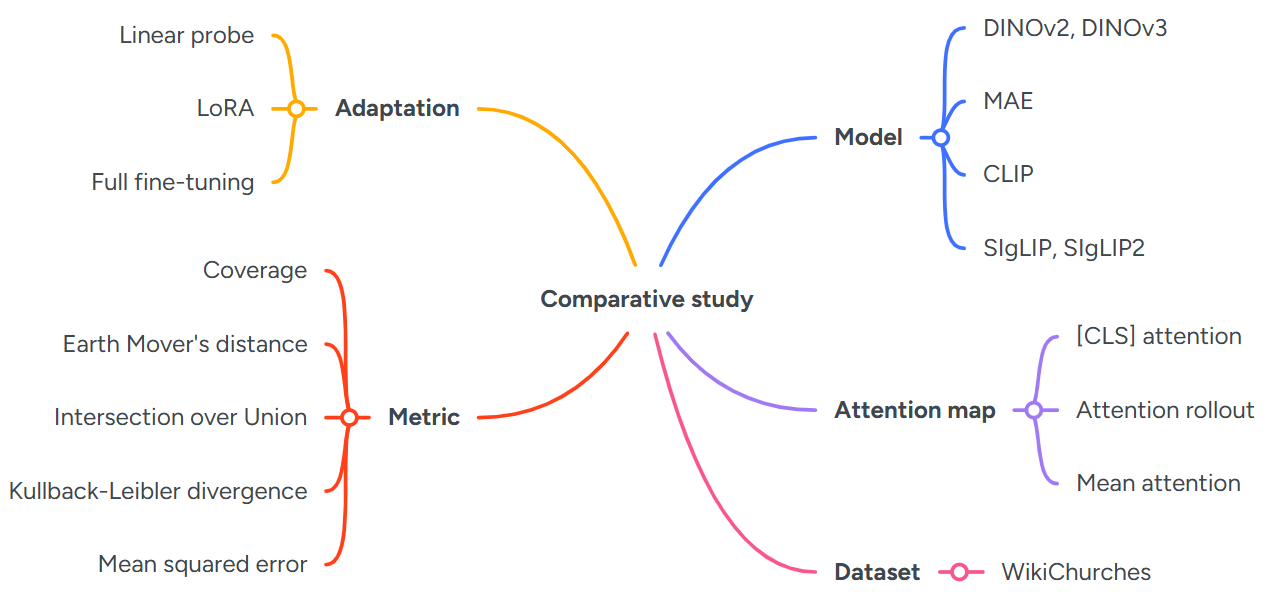
\includegraphics[width=\textwidth]{framework_v2.png}
\caption{Our comparative study compares 6 vision foundation models, 3 types of attention maps, 3 model adaptation strategies, and 5 performance metrics on 1 benchmark dataset. \label{figure framework overview}}
\end{figure}

\subsection{Dataset}

The image dataset used in this study is the WikiChurches benchmark dataset~\cite{Barz21WikiChurches}, which is a fine-grained architectural-style dataset of European church buildings. Its annotation file defines 106 architectural feature types, including arches, windows, towers, and portals, and provides bounding-box annotations with normalized coordinates.

This study uses two data scopes. First, we use an expert-annotated evaluation subset containing 139 images and 631 bounding boxes across four architectural styles: Romanesque~(51 images), Gothic~(49 images), Renaissance~(22 images), and Baroque~(17 images). This subset is used exclusively for evaluation, mainly of attention alignment and, in Section~\ref{section RQ3 correctness}, of classification correctness. Second, for downstream fine-tuning, we draw from the larger WikiChurches style-labelled metadata release but restrict training to primary images whose metadata maps directly to the same four target styles. Under this four-style setting, the candidate fine-tuning pool contains 4,713 labelled primary images. All 139 expert-annotated evaluation image IDs are treated as held out from training; 125 of these IDs overlap the metadata-derived candidate pool, while the remaining 14 are assigned more specific or adjacent metadata labels outside the four exact target classes, such as Brick Gothic, French Gothic, English Gothic, Norman Architecture, Gothic Revival, or Spanish Renaissance. Removing the 125 overlapping evaluation images leaves 4,588 images for the train-validation split. The image examples are illustrated in Figure \ref{figure wikichurches overview}.


\begin{figure}[!h]
\centering
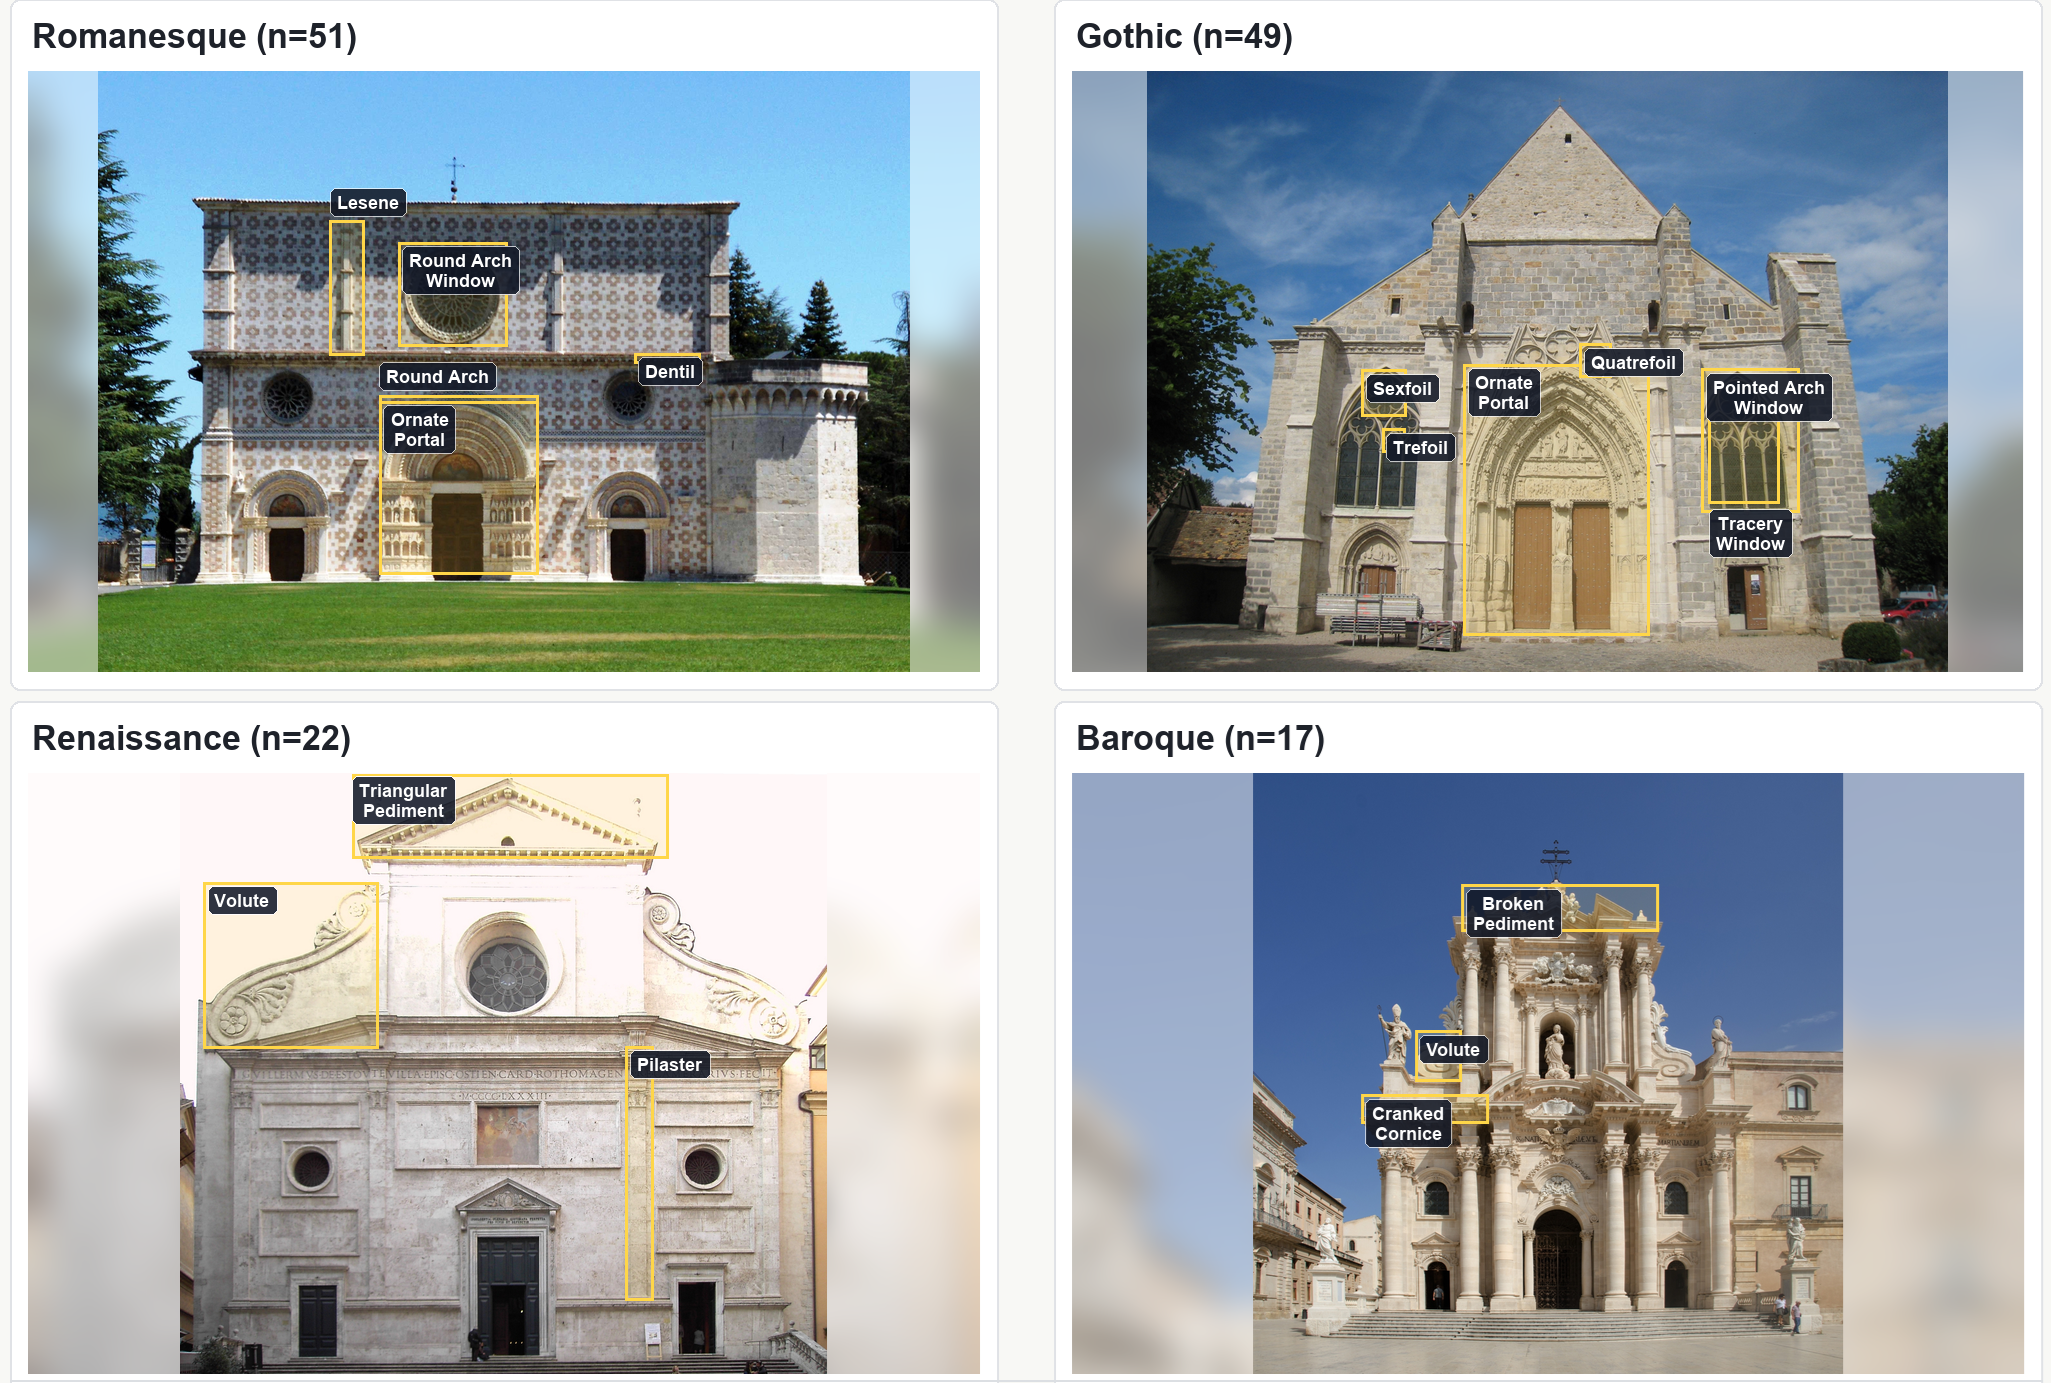
\includegraphics[width=\textwidth]{wikichurches_overview_v1.png}
\caption{Representative images from the expert-annotated WikiChurches evaluation subset for the four architectural styles used in this study: Romanesque (51 images), Gothic (49 images), Renaissance (22 images), and Baroque (17 images). Yellow boxes denote expert-annotated building parts, and dark labels indicate the corresponding architectural feature annotations.}
\label{figure wikichurches overview}
\end{figure}


\subsection{Vision foundation models studied in this paper}

This paper compares six vision foundation models spanning image-only self-supervised models and vision-language models. The image-only models include DINOv2~\cite{Oquab24DINOv2}, DINOv3~\cite{Simeoni26DINOv3}, and MAE~\cite{He22MAE}. The vision-language models include CLIP~\cite{Radford21CLIP}, SigLIP~\cite{Zhai23SigLIP}, and SigLIP2~\cite{Tschannen25SigLIP2}; for these models, only their visual encoders are analyzed. DINOv2 uses a patch size of~14, producing a $16\times16$ spatial grid with four register tokens. All other models use a patch size of~16, producing a $14\times14$ spatial grid.

We extract attention maps with one of two methods, depending on the model, as summarized in Table~\ref{table attention method list}. DINOv2, DINOv3, MAE, and CLIP provide a \texttt{[CLS]}-token pathway, so we use the attention from the \texttt{[CLS]} token to the patch tokens. SigLIP and SigLIP2 do not provide an equivalent \texttt{[CLS]}-token pathway, so we use a mean-attention proxy, defined as the average attention that each patch receives from all patches. The proxy is computed from the encoder layers and does not use the attention weights of the pooling head that produces the pooled SigLIP representation.


\begin{table}[!th]
\centering \caption{A list of attention extraction methods used in this study. \label{table attention method list}}
\begin{tabular}{ccc}
\toprule
Attention method & Vision foundation model & Remark \\ \midrule
\texttt{[CLS]} attention & DINOv2, DINOv3, MAE, CLIP & Native \texttt{[CLS]} token \\
Mean attention & SigLIP, SigLIP2 & Proxy (no \texttt{[CLS]} token) \\
\bottomrule
\end{tabular}
\end{table}

We compare three model adaptation strategies. First, in the \textit{linear probe setting}, the pretrained backbone is frozen, and only a newly added classification head is trained, providing a lightweight evaluation of the separability of the frozen representations. Second, in the \textit{LoRA setting}, low-rank trainable adapters are inserted into selected layers while the original backbone parameters remain frozen, enabling parameter-efficient adaptation. Third, in the \textit{full fine-tuning setting}, all model parameters are updated on the downstream task, allowing the entire visual representation to be optimized for architectural style recognition.

\subsection{Performance metrics for attention alignment}

To quantify the alignment between model attention and expert annotations, we need to convert the expert-annotated bounding boxes for each image into a single target map. This allows the model attention map and the expert annotations to be compared at the same spatial resolution. Furthermore, we consider two types of maps, including the binary union mask of expert-annotated boxes and the Gaussian soft-union target map constructed from the same boxes. We use both these two because they capture complementary notions of alignment. The binary mask provides a strict region-level reference for evaluating whether high-attention pixels fall inside expert-annotated architectural parts, whereas the soft target provides a dense spatial reference that accounts for the center, scale, and spatial spread of each annotated region.

For each image, we construct a Gaussian soft-union target map (denoted as $G$) from its expert-annotated bounding boxes as follows. Let the $i$-th expert-annotated box be represented by normalized corner coordinates $(\mathrm{left}_i, \mathrm{top}_i, \mathrm{right}_i, \mathrm{bottom}_i) \in [0, 1]$. Given an attention map of width $W$ and height $H$, the box coordinates are mapped to the heatmap resolution by computing the box center and spatial extent as
\begin{equation}
c_{i,x} = \frac{\mathrm{left}_i + \mathrm{right}_i}{2}W,
\quad
c_{i,y} = \frac{\mathrm{top}_i + \mathrm{bottom}_i}{2}H,
\end{equation}
\begin{equation}
w_i = \max\left(\left(\mathrm{right}_i - \mathrm{left}_i\right)W, 1\right),
\quad
h_i = \max\left(\left(\mathrm{bottom}_i - \mathrm{top}_i\right)H, 1\right),
\end{equation}
where $c_{i,x}$ and $c_{i,y}$ denote the box center in pixels, and $w_i$ and $h_i$ denote the box width and height in pixels. Then, we place an axis-aligned anisotropic 2-D Gaussian at each
box centre. The per-axis standard deviations are set according to the box size as
\begin{equation}
\sigma_{i,x} = \max\left(\frac{w_i}{4}, 1\right),
\qquad
\sigma_{i,y} = \max\left(\frac{h_i}{4}, 1\right).
\end{equation}
The purpose of the Gaussian is to turn each box into a continuous map, so that attention just outside an annotated region is penalized less than attention far from it. With $\sigma = w_i/4$, the box edges lie $2\sigma$ from the centre, so about 95\% of the Gaussian's mass along each axis, and about 91\% in two dimensions, falls inside the box, while the target value at the box edge is $e^{-2} \approx 0.14$ rather than zero. Tying $\sigma$ to the width and height of each box keeps this spread the same relative to the box for large and small elements and preserves the box's aspect ratio. The lower bound of one pixel prevents very small boxes from collapsing to a single-pixel spike; on the $224 \times 224$ grid it applies to 28 of the 631 boxes along at least one axis. The value of $\sigma$ was fixed in advance and not tuned, and it affects only the MSE, KL divergence and EMD metrics, since IoU@90 and Coverage use the binary mask.
The resulting per-box Gaussian map ($G_i$) is peak-normalized to one as
\begin{equation}
G_i(x, y) = \exp\left[-\frac{(x - c_{i,x})^{2}}{2\sigma_{i,x}^{2}}-\frac{(y - c_{i,y})^{2}}{2\sigma_{i,y}^{2}}\right].
\end{equation}
When an image contains multiple expert-annotated boxes, the per-box maps are combined using a pixel-wise maximum, forming a soft union over all annotated regions. The resulting final per-image map is then normalized to obtain
\begin{equation}
G(x, y) = \frac{\max_{i} G_i(x, y)}{\max_{x, y} \max_{i} G_i(x, y)}.
\end{equation}


Let $A$ denote the attention map obtained from a vision foundation model, and let $M$ denote the union binary mask of expert-annotated boxes, and $G$ is the Gaussian soft-union target map constructed from the same boxes. The following five metrics are computed between $A$, $M$, and $G$ to evaluate attention alignment.

\begin{itemize}
\item \textit{Intersection over Union} (IoU). It thresholds $A$ by selecting the top-$K$ pixels using \texttt{torch.topk}, and then computes overlap between the resulting binary attention mask and $M$ as
\begin{equation}
\mathrm{IoU} = \frac{|\hat{A} \cap M|}{|\hat{A} \cup M|},
\end{equation}
where $\hat{A}$ is the binary mask containing the $K$ pixels with the highest attention values. In our study, $K$ is set to $10\%$ of the total number of heatmap pixels. This is equivalent to thresholding $A$ at the $90$-th percentile of attention values. Therefore, we denote this metric as IoU@90. A higher IoU@90 value indicates better alignment performance.

We report the 90th percentile because the expert-annotated regions are small. Their union covers less than 10\% of the image in 102 of the 139 images (Section~\ref{section RQ1 results}). For these images, a lower percentile selects even more pixels than the annotations cover, which lowers the highest IoU they can reach. Because $K$ is a fixed share of pixels rather than a fixed attention value, every model is scored on the same number of pixels, regardless of its patch grid or the scale of its attention values. We also computed IoU at the 50th, 60th, 70th, 75th, 80th, and 85th percentiles. Among the frozen models, each at its best layer, DINOv3 and DINOv2 rank first and second and SigLIP2 ranks last at every threshold, whereas the order of SigLIP, MAE, and CLIP changes. We therefore report only IoU@90 and use Coverage, which needs no threshold, as a complementary measure.

\item \textit{Coverage}. It measures the fraction of total attention energy inside that falls inside the mask $M$ as
\begin{equation}
\text{Coverage} = \frac{\sum_{i \in M} A_i}{\sum_i A_i}.
\end{equation}
A higher Coverage value indicates that more attention mass is assigned to expert-annotated regions.

\item \textit{Mean Squared Error} (MSE). It measures the pixel-wise squared difference between the attention map $A$ and the Gaussian soft target $G$ as
\begin{equation}
\mathrm{MSE} = \frac{1}{N}\sum_{i=1}^{N}\left(A_i - G_i\right)^{2}.
\end{equation}
A lower MSE value indicates better pixel-level agreement with the soft expert target.

\item \textit{Kullback-Leibler} (KL) divergence \cite{Kullback1951}. It measures the distributional discrepancy between the Gaussian soft target $G$ and the model attention map $A$ as
\begin{equation}
\mathrm{KL}(G \| A) = \sum_{i=1}^{N} G_i \log\frac{G_i}{A_i}.
\end{equation}
A lower KL divergence indicates that the model's attention distribution is closer to the expert-derived target distribution.

\item \textit{Earth Mover's Distance} (EMD). \cite{Rubner2000}. It measures the spatial cost of transforming the model's attention distribution into the expert-derived distribution. We compute the $1$-Wasserstein distance between $A$ and $G$ after bilinearly downsampling both maps to a shared $8 \times 8$ grid and re-normalizing them to unit mass. Euclidean distance between normalized grid-cell centers is used as the ground cost as
\begin{equation}
\mathrm{EMD}(A, G) = \min_{\pi \in \Pi(A, G)}\sum_{i,j} \pi_{ij} \|c_i - c_j\|_2,
\end{equation}
where $\Pi(A, G)$ is the set of joint distributions with marginals $A$ and $G$, and $c_i, c_j$ are the normalized coordinates of grid cells $i$ and $j$. A lower EMD value indicates better spatial distributional alignment.
\end{itemize}

These metrics catch different failure modes of attention alignment. IoU@90 evaluates whether the most highly attended pixels fall inside expert-annotated regions, while Coverage measures how much total attention energy is assigned to those regions. MSE, KL divergence, and EMD compare the full attention map against the Gaussian soft-union target, revealing cases where the attention map may partially overlap with expert annotations but still differs in spatial concentration, distributional shape, or mass displacement.

\subsection{Statistical analysis}

All statistical analyses use the image as the unit of analysis. For paired comparisons between two conditions $A$ and $B$ evaluated on the same annotated images, we define the $i$-th image-level paired difference as $d_i=x_i^A-x_i^B$. We test whether the mean paired difference differs from zero using the paired $t$-test \cite{SciPy}, $t=\bar d/(s_d/\sqrt n)$, when the $n$ paired differences are adequately modelled by a normal distribution with a mean $\bar d$ and a standard deviation $s_d$. Otherwise, we use the Wilcoxon signed-rank test \cite{SciPy}. To distinguish effect magnitude from statistical significance, we also report the paired Cohen's effect size \cite{Cohen1988, Lakens2013}, $d_z=\bar d/s_d$. For estimation uncertainty, we report 95\% bootstrap confidence intervals for mean shifts by resampling the paired image-level differences \cite{SciPy}. For multiple testing, $p$-values are adjusted within each metric family using Holm's sequential multiple-comparison correction \cite{Holm1979}. For analyses that are not paired two-condition comparisons, we use nonparametric and correlation-based tests according to the analysis objective. Specifically, Kruskal-Wallis tests ~\cite{SciPy} are used to assess whether $\Delta$IoU@90 differs across architectural styles. Pearson's $r$ is used to measure linear association between per-image score vectors, while Spearman's $\rho$ is used to measure rank-based association~\cite{SciPy}.


\section{Experimental results} \label{section results}

\subsection{Implementation details}

The WikiChurches benchmark dataset~\cite{Barz21WikiChurches} was divided into two non-overlapping subsets. The expert-annotated evaluation subset contains 139 images with 631 bounding-box annotation instances drawn from a 106-type architectural-feature ontology. The primary-style distribution is 51 Romanesque images with 217 boxes, 49 Gothic images with 290 boxes, 22 Renaissance images with 93 boxes, and 17 Baroque images with 31 boxes. This gives an average of 4.54 expert-annotated boxes per image overall. This subset was used only for evaluation, of attention alignment and of classification correctness (Section~\ref{section RQ3 correctness}), and was excluded from all downstream training and validation splits.

The annotation file organizes the 631 boxes into 566 groups. Most groups contain a single box, while the 60 groups with several boxes describe a composite element through its parts; for example, a tracery window may be annotated with separate boxes for the pointed-arch window, its tracery, and a trefoil. We used the feature label of each individual box rather than the group label. Boxes can overlap, both within and across groups. Of the 1,420 pairs of boxes in the same image, 136 overlap, and in 54 of these one box lies entirely inside the other; such overlaps occur in 66 of the 139 images. Images contain 1 to 10 boxes (median 4), and the union of an image's boxes covers 0.4\% to 30.8\% of the image (median 4.8\%). Overlapping pixels are counted once in the binary union mask and take the pixel-wise maximum in the Gaussian target, so a region annotated twice receives no extra weight. In the feature-level analysis, each box is scored separately.

The 139 evaluation images are JPEG files of varying size, from 414 to 2,281 pixels wide and 450 to 2,142 pixels high (median width and median height both 1,280 pixels), with width-to-height ratios between 0.60 and 1.78. All images were loaded in RGB format. For attention-alignment evaluation, each image was resized directly to $224 \times 224$ pixels without cropping, using each model's default interpolation (bicubic for DINOv2, CLIP, and SigLIP; bilinear for DINOv3, MAE, and SigLIP2). This resize changes the aspect ratio of non-square images, but it retains the full image extent, so no annotated region is excluded by cropping. The WikiChurches bounding boxes are stored as normalized coordinates relative to the original image dimensions. During evaluation, each box was rasterized on the same full-image $224 \times 224$ grid and converted into a binary mask, so the attention maps and the expert masks share one coordinate frame. Multiple boxes from the same image were combined into a single union mask for overlap-based metrics. Negative normalized coordinates in the annotation file were clamped to zero before mask generation. Model attention maps were computed at the native patch-grid resolution of each backbone and then upsampled to $224 \times 224$ using bilinear interpolation. Each upsampled map was min-max normalized to $[0,1]$ on a per-image basis. DINOv2 uses $14 \times 14$ patches, giving a $16 \times 16$ patch grid for $224 \times 224$ inputs. DINOv3, MAE, CLIP, SigLIP, and SigLIP2 use $16 \times 16$ patches, giving a $14 \times 14$ patch grid. For EMD, both the attention map and target distributions were additionally resized to a shared $8 \times 8$ support before the transport-distance computation.

For downstream adaptation, we used four architectural style classes, including Romanesque, Gothic, Renaissance, and Baroque. Images without one of these four labels were excluded from style-classification training. The primary experiment used a shared stratified train-validation split with random seed 42. After removing the 125 expert-annotated evaluation images, the training split contained 3,671 images, and the validation split contained 917 images. The training split contained 1,214 Romanesque, 1,216 Gothic, 137 Renaissance, and 1,104 Baroque images; the validation split contained 303 Romanesque, 304 Gothic, 34 Renaissance, and 276 Baroque images. The same split was used for all models and adaptation strategies.

Pretrained model weights were loaded from Hugging Face checkpoints: DINOv2 from \texttt{facebook/dinov2-with-registers-base}, DINOv3 from \texttt{facebook/dinov3-vitb16-pretrain-lvd1689m}, MAE from \texttt{facebook/vit-mae-base}, CLIP from \texttt{openai/clip-vit-base-patch16}, SigLIP from \texttt{google/siglip-base-patch16-224}, and SigLIP2 from \texttt{google/siglip2-base-patch16-224}. All six models use ViT-Base-scale visual backbones with 12 transformer layers, 12 attention heads, and 768-dimensional hidden states. For CLIP, SigLIP, and SigLIP2, only the visual encoder was used.

We evaluated three model adaptation settings, including linear probing, LoRA adaptation, and full fine-tuning. In the linear-probe setting, the pretrained backbone was frozen, and a newly initialized four-class linear classifier was trained on top of the frozen representation. For DINOv2, DINOv3, MAE, and CLIP, the classifier used the \texttt{[CLS]}-token representation. For SigLIP and SigLIP2, which do not expose an equivalent \texttt{[CLS]}-token pathway, the classifier used the pooled visual representation. In the LoRA setting, the pretrained backbone weights remained frozen except for low-rank adapters inserted into the attention query and value projection layers. LoRA used rank 8, alpha 32, dropout 0.1, and no bias adaptation. For the 12-layer, 768-dimensional ViT-Base backbones used here, this corresponds to 294,912 trainable adapter parameters per backbone. The four-class classifier adds 3,076 trainable parameters. DINOv2 and MAE used the \texttt{query} and \texttt{value} target modules, while DINOv3, CLIP, SigLIP, and SigLIP2 used \texttt{q\_proj} and \texttt{v\_proj}. In the full fine-tuning setting, both the backbone parameters and the classification head were updated.

All training runs used the AdamW optimizer with class-weighted cross-entropy to account for style imbalance. The batch size was 16, weight decay was 0.01, and training lasted for 3 epochs. The classifier-head learning rate was set to $1 \times 10^{-3}$ in all settings. The backbone learning rate was $1 \times 10^{-5}$ for full fine-tuning and $1 \times 10^{-4}$ for LoRA. The learning-rate schedule used linear warmup for 10\% of training steps, followed by cosine decay. Gradients were clipped to a maximum norm of 1.0. Training images were augmented using random resized crop to $224 \times 224$ with a scale range of $0.8$-$1.0$, random horizontal flipping with probability 0.5, and color jitter with brightness and contrast set to 0.2. Validation and attention-alignment evaluation used deterministic preprocessing and did not include these random augmentations. Training and validation images were passed through each model's native Hugging Face preprocessing, which for DINOv2 and CLIP includes a central $224 \times 224$ crop. Checkpoints were selected on validation accuracy under this preprocessing, and attention maps from all checkpoints were then extracted with the full-image resize described above.

For each model-strategy run, we selected the checkpoint with the highest classification accuracy on the shared non-annotated validation split. The selected checkpoint was then evaluated on the untouched 139-image expert-annotated subset for attention alignment. Except for the layer-head analysis in Figure~\ref{figure RQ3 head ranking}, RQ3 measures alignment at the final transformer layer (layer 11), whose output feeds the classifier, rather than at the best layer selected separately for each metric in RQ1 (Table~\ref{table RQ1 result}). The experiment consists of 18 runs, corresponding to six models and three adaptation strategies. The selected epochs came from epochs 1 through 3, depending on the model and adaptation strategy, but every run was trained for the same maximum of 3 epochs. To relate classification correctness to attention alignment (Section~\ref{section RQ3 correctness}), each selected checkpoint also classified the 139 evaluation images with the same native preprocessing as validation. For the frozen models, these predictions come from the linear-probe checkpoint, whose backbone is frozen and therefore produces the frozen model's attention. The true style of each evaluation image is its primary style in the expert annotation file, which differs from the WikiChurches metadata label used for training and validation for 4 of the 139 images.

All experiments were implemented in Python 3.12.11 using PyTorch 2.10.0. Experiments were conducted on a MacBook Pro with an Apple M4 Pro chip, 14-core CPU, 20-core integrated GPU, and 48 GB unified memory. The PyTorch MPS backend was used when available; CUDA was not available in this environment.

\subsection{Results from RQ1: the final attention alignment of frozen pretrained models}\label{section RQ1 results}

For RQ1, we evaluate attention alignment in frozen pretrained models before any task-specific adaptation.

Table~\ref{table RQ1 result} summarizes the results obtained using the five performance metrics. Overall, DINOv3 achieves the strongest frozen-model alignment. It obtains the best performance on IoU@90, Coverage, KL divergence, and EMD, indicating that its attention maps overlap more strongly with expert-annotated architectural regions and are also closer to the expert annotations at the distributional level. However, DINOv3 does not achieve the lowest MSE. Instead, SigLIP2 obtains the best MSE score, followed closely by SigLIP. This difference suggests that attention alignment should not be reduced to a single metric: a model may produce locally smooth attention maps with low pixel-wise error while still placing attention mass in less accurate spatial locations.

\begin{table}[!h]
\centering
\caption{Results from RQ1: Frozen-model alignment using the best default-method layer selected separately for each metric.\label{table RQ1 result}}
\begin{tabular}{cccccc}
\toprule
Vision foundation model & IoU@90 $\uparrow$ & Coverage $\uparrow$ & MSE $\downarrow$ & KL divergence $\downarrow$ & EMD $\downarrow$ \\ \midrule
DINOv2    & 0.118 & 0.128 & 0.021 & 2.376 & 0.271 \\
DINOv3     & 0.133 & 0.137 & 0.027 & 2.325 & 0.260 \\
MAE        & 0.070 & 0.090 & 0.048 & 2.756 & 0.318 \\
CLIP      & 0.051 & 0.088 & 0.021 & 2.853 & 0.323 \\
SigLIP    & 0.074 & 0.076 & 0.018 & 3.002 & 0.348 \\
SigLIP2   & 0.047 & 0.071 & 0.017 & 3.071 & 0.354 \\ \bottomrule
\end{tabular}
\end{table}

Among the remaining models, DINOv2 ranks second on IoU@90, Coverage, KL divergence, and EMD, close behind DINOv3 (0.118 versus 0.133 on IoU@90), demonstrating relatively strong spatial localization among the frozen models. MAE performs moderately on IoU@90 and Coverage but has the highest MSE, indicating weaker pixel-level agreement with expert annotations. CLIP shows relatively low IoU@90 and Coverage, indicating limited spatial overlap between its frozen attention maps and expert-annotated regions. SigLIP and SigLIP2 achieve the lowest MSE values, but their higher KL divergence and EMD scores indicate that their attention distributions remain less well aligned with expert annotations despite favorable pixel-wise error.

These cross-model comparisons mix the two extraction methods listed in Table~\ref{table attention method list}. DINOv2, DINOv3, MAE, and CLIP are scored on their \texttt{[CLS]}-token attention, whereas SigLIP and SigLIP2 are scored on the mean-attention proxy. The two maps measure different quantities, so the differences between the SigLIP models and the other four, including the lower MSE of the SigLIP models, may partly reflect the extraction method rather than the model. This applies to every comparison between the two groups, including Tables~\ref{table RQ1 result} and~\ref{table RQ1 feature categories} and Figures~\ref{figure RQ2 layer ranking} and~\ref{figure RQ3 accuracy alignment}. Comparisons within a model, such as across layers or between frozen and adapted versions, and comparisons between SigLIP and SigLIP2 use a single method and are not affected.

Since DINOv3 achieves the strongest overall attention alignment, as shown in Table~\ref{table RQ1 result}, we further examine whether its advantage is consistent with its model design. We hypothesize that DINOv3 benefits from the combination of large-scale self-supervised training and a training recipe intended to preserve dense spatial representations. The DINOv3 technical report~\cite{Simeoni26DINOv3} identifies dense-feature degradation as a potential failure mode during long self-supervised training and introduces Gram anchoring to stabilize patch-level feature maps. Because the RQ1 metrics explicitly measure spatial correspondence between the model attention map and expert-annotated architectural regions, a training strategy designed to preserve dense features provides a plausible explanation for DINOv3's stronger alignment.

To further assess this explanation, we conduct two additional checks, summarized in Table~\ref{table RQ1 dinov3}. The first check evaluates robustness. Paired image-level comparisons against the next-best model, DINOv2, show that DINOv3 outperforms it on all metrics except MSE, with Holm-adjusted $p \le 0.006$ (Wilcoxon signed-rank test over the 139 images, each model at its best layer). This indicates that the observed advantage is not merely a leaderboard artifact caused by aggregation over images, although the margin over DINOv2 is small. The second check examines where DINOv3 performs best. If DINOv3 preserves cleaner patch-level spatial structure, its attention should align more strongly with mid-scale to large-scale architectural elements while remaining less effective for small ornamental details. This expectation matches our observations: DINOv3 performs best on visually prominent styles such as Gothic and Romanesque, aligns strongly with large coherent features such as Ornate Portals and Tracery Roses, and scores lowest on small decorative elements such as Crockets and Pinnacles, whose small box areas also limit their attainable IoU@90. The last three rows in Table \ref{table RQ1 dinov3} summarize where frozen DINOv3’s attention aligns best or worst with expert annotations: it scores highest on visually prominent structural styles/features and lowest on small ornamental details.

\begin{table}[!h]
\centering
\caption{Additional robustness and spatial checks for DINOv3. For lower-is-better metrics, the reported gap is computed as the next-best model score minus the DINOv3 score.\label{table RQ1 dinov3}}
\begin{tabular}{lp{0.3\textwidth}p{0.35\textwidth}}
\toprule
Check & Result & Finding \\ \midrule
Paired performance gap & $+0.0150$ (IoU@90), $+0.0097$ (Coverage), $+0.0515$ (KL divergence), $+0.0111$ (EMD) & DINOv3's lead is not an aggregation artifact. \\
Strongest styles & Gothic: 0.169 (IoU@90); Romanesque: 0.160 (IoU@90) & Alignment is highest for visually prominent structural styles. \\
Strongest features & Ornate Portal: 0.214 (IoU@90); Tracery Rose: 0.164 (IoU@90) & Attention aligns well with large, coherent architectural parts. \\
Weakest features & Crocket; Fleuron; Pinnacle & These are the smallest annotated parts, so their attainable IoU@90 is low. \\
\bottomrule
\end{tabular}
\end{table}

Because an image can contain several annotated regions, we also examined how frozen alignment depends on the number of boxes per image and on the fraction of the image covered by their union. For each model at its best IoU@90 layer, per-image IoU@90 increased with the union area (Spearman $\rho$ from $+0.28$ for MAE to $+0.60$ for CLIP) and with the number of boxes ($\rho$ from $+0.22$ for SigLIP2 to $+0.45$ for SigLIP), with Holm-adjusted $p < 0.01$ across the six models in both cases. Part of this trend follows from the metric itself. IoU@90 keeps a fixed 10\% of pixels, so for an image whose annotations cover a fraction $g<0.1$ of the image, the attainable IoU@90 is at most $g/0.1$. This bound applies to 102 of the 139 images. It also applies to individual boxes: at their median box size, Crocket, Fleuron, and Pinnacle boxes can reach at most 0.002, 0.005, and 0.019, respectively.

Table~\ref{table RQ1 feature categories} extends the feature-level analysis to all six models by grouping feature types under their top-level categories in the WikiChurches ontology. Arch and window boxes have similar median areas (0.67\% and 0.74\% of the image), so their IoU@90 values are directly comparable. Five of the six models align better with windows than with arches, although the difference is small for MAE, whereas SigLIP aligns better with arches. Portals give the highest IoU@90 for DINOv2, DINOv3, MAE, and SigLIP, pediments for CLIP, and tracery for SigLIP2. Ornaments and pinnacles, the two smallest categories, are among the three lowest-scoring categories for every model, which is consistent with the area bound above.

\begin{table}[!h]
\centering
\caption{Frozen-model IoU@90 by top-level architectural category. Each box counts under every top-level ontology type that its feature descends from, so boxes such as round-arch windows count as both arches and windows. Only categories with at least 20 boxes are shown. Area is the median box area as a percentage of the image. Each model uses its best IoU@90 layer, as in Table~\ref{table RQ1 result}.\label{table RQ1 feature categories}}
\begin{tabular}{lrrcccccc}
\toprule
Category & Boxes & Area (\%) & DINOv2 & DINOv3 & MAE & CLIP & SigLIP & SigLIP2 \\ \midrule
Arch     & 177 & 0.67 & 0.041 & 0.045 & 0.031 & 0.013 & 0.038 & 0.018 \\
Window   & 161 & 0.74 & 0.052 & 0.062 & 0.032 & 0.018 & 0.030 & 0.025 \\
Column   &  88 & 1.29 & 0.030 & 0.043 & 0.025 & 0.013 & 0.036 & 0.009 \\
Ornament &  85 & 0.13 & 0.012 & 0.008 & 0.003 & 0.004 & 0.002 & 0.004 \\
Blind    &  58 & 0.56 & 0.027 & 0.030 & 0.015 & 0.010 & 0.010 & 0.008 \\
Tracery  &  53 & 1.17 & 0.085 & 0.103 & 0.036 & 0.024 & 0.033 & 0.038 \\
Portal   &  47 & 4.03 & 0.090 & 0.115 & 0.091 & 0.026 & 0.141 & 0.030 \\
Pediment &  44 & 2.48 & 0.026 & 0.032 & 0.014 & 0.047 & 0.014 & 0.027 \\
Frieze   &  34 & 0.28 & 0.013 & 0.015 & 0.004 & 0.003 & 0.002 & 0.005 \\
Pinnacle &  28 & 0.19 & 0.005 & 0.005 & 0.001 & 0.003 & 0.002 & 0.002 \\
Cornice  &  21 & 1.82 & 0.027 & 0.020 & 0.007 & 0.029 & 0.007 & 0.004 \\ \bottomrule
\end{tabular}
\end{table}


\subsection{Results from RQ2: the internal attention alignment across layers and heads}

For RQ2, we assess whether intermediate layers and attention heads exhibit feature-specific specialization for different architectural elements. 

\subsubsection{A study on various layers}

To evaluate how attention alignment varies across models' depth, we plot the IoU@90 performance of each model at every transformer layer in Figure~\ref{figure RQ2 layer ranking}. The layer-wise trends show significant differences across pretrained models. DINOv3 exhibits the clearest late-layer improvement, rising sharply after layer 6 and reaching the highest alignment at the final layer. DINOv2 follows a similar late-layer pattern. Its IoU@90 rises from 0.063 at layer 6 to 0.111 at layer 7 and reaches 0.118 at the final layer, briefly exceeding DINOv3 at layers 8 and 9. In contrast, CLIP peaks in the earliest layers and declines substantially afterward, which indicates that its later visual representations are less spatially aligned with expert-annotated regions. MAE fluctuates between 0.031 and 0.070 across layers and reaches its highest value at the final layer, while SigLIP and SigLIP2 show more irregular patterns with isolated mid-layer peaks. 

\begin{figure}[!h]
\centering
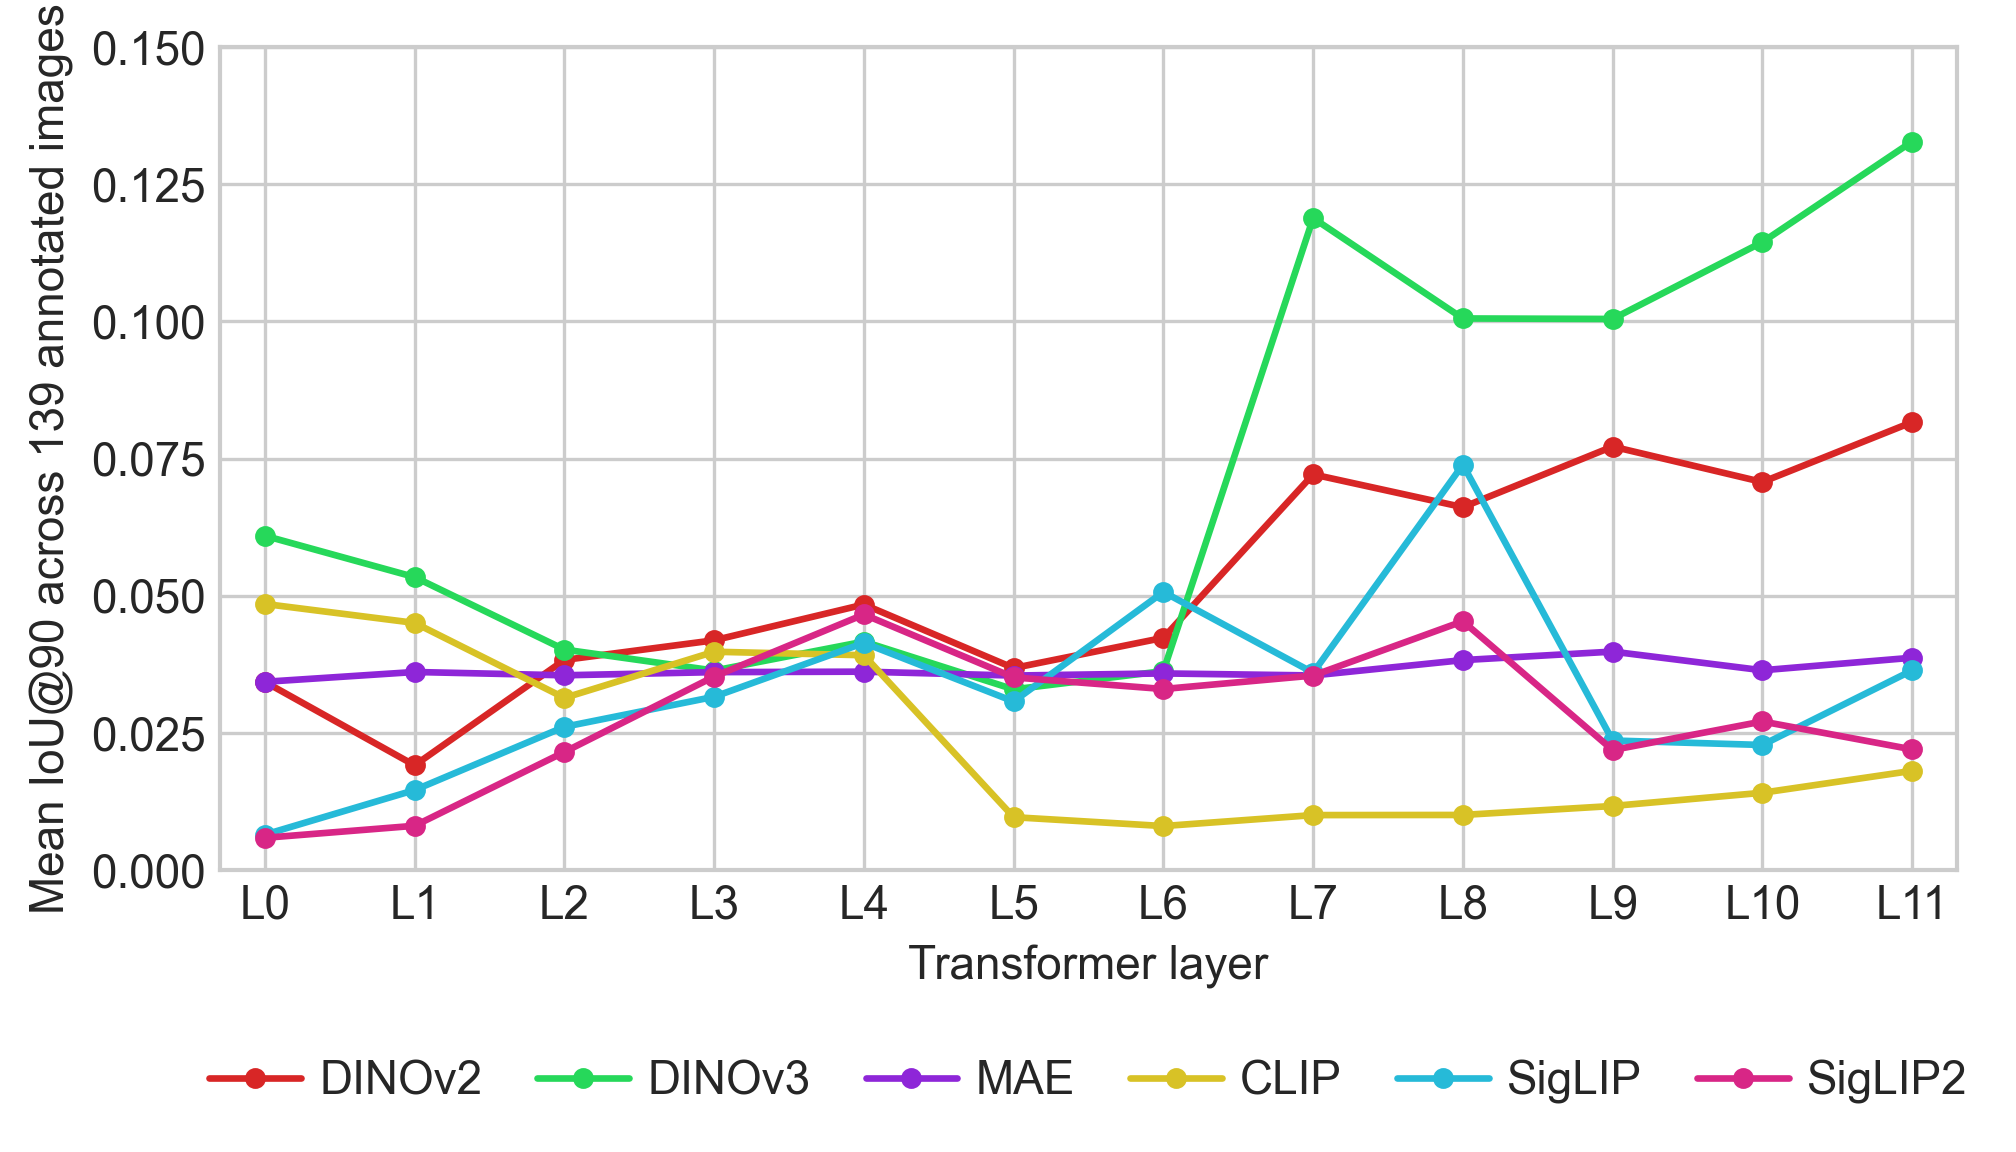
\includegraphics[width=\linewidth]{RQ2_layer_iou_new.png}
\caption{Layer-wise attention alignment with expert annotations. The mean IoU@90 performance across the 139 expert-annotated images is reported for each transformer layer.\label{figure RQ2 layer ranking}}
\end{figure}

\subsubsection{A study on various heads}

To evaluate head-level behavior, we conduct two experiments. The first experiment uses the \textit{head-feature matrix} to examine which architectural features individual attention heads align with. Figure~\ref{figure rq2_head_feature_matrix} shows a representative example for the frozen DINOv3 model at layer~10, based on IoU@90 as the alignment metric. The dominant head, H8, is highlighted. The colour scale is encoded in the figure, where lighter cells indicate weaker expert-annotated box alignment, and darker cells indicate stronger expert-annotated box alignment. The rows with the strongest H8 alignment correspond mainly to portal-scale and facade-scale structures. This pattern supports the observation that the strongest heads align more clearly with large, coherent architectural parts than with small decorative details.

\begin{figure}[!ht]
\centering
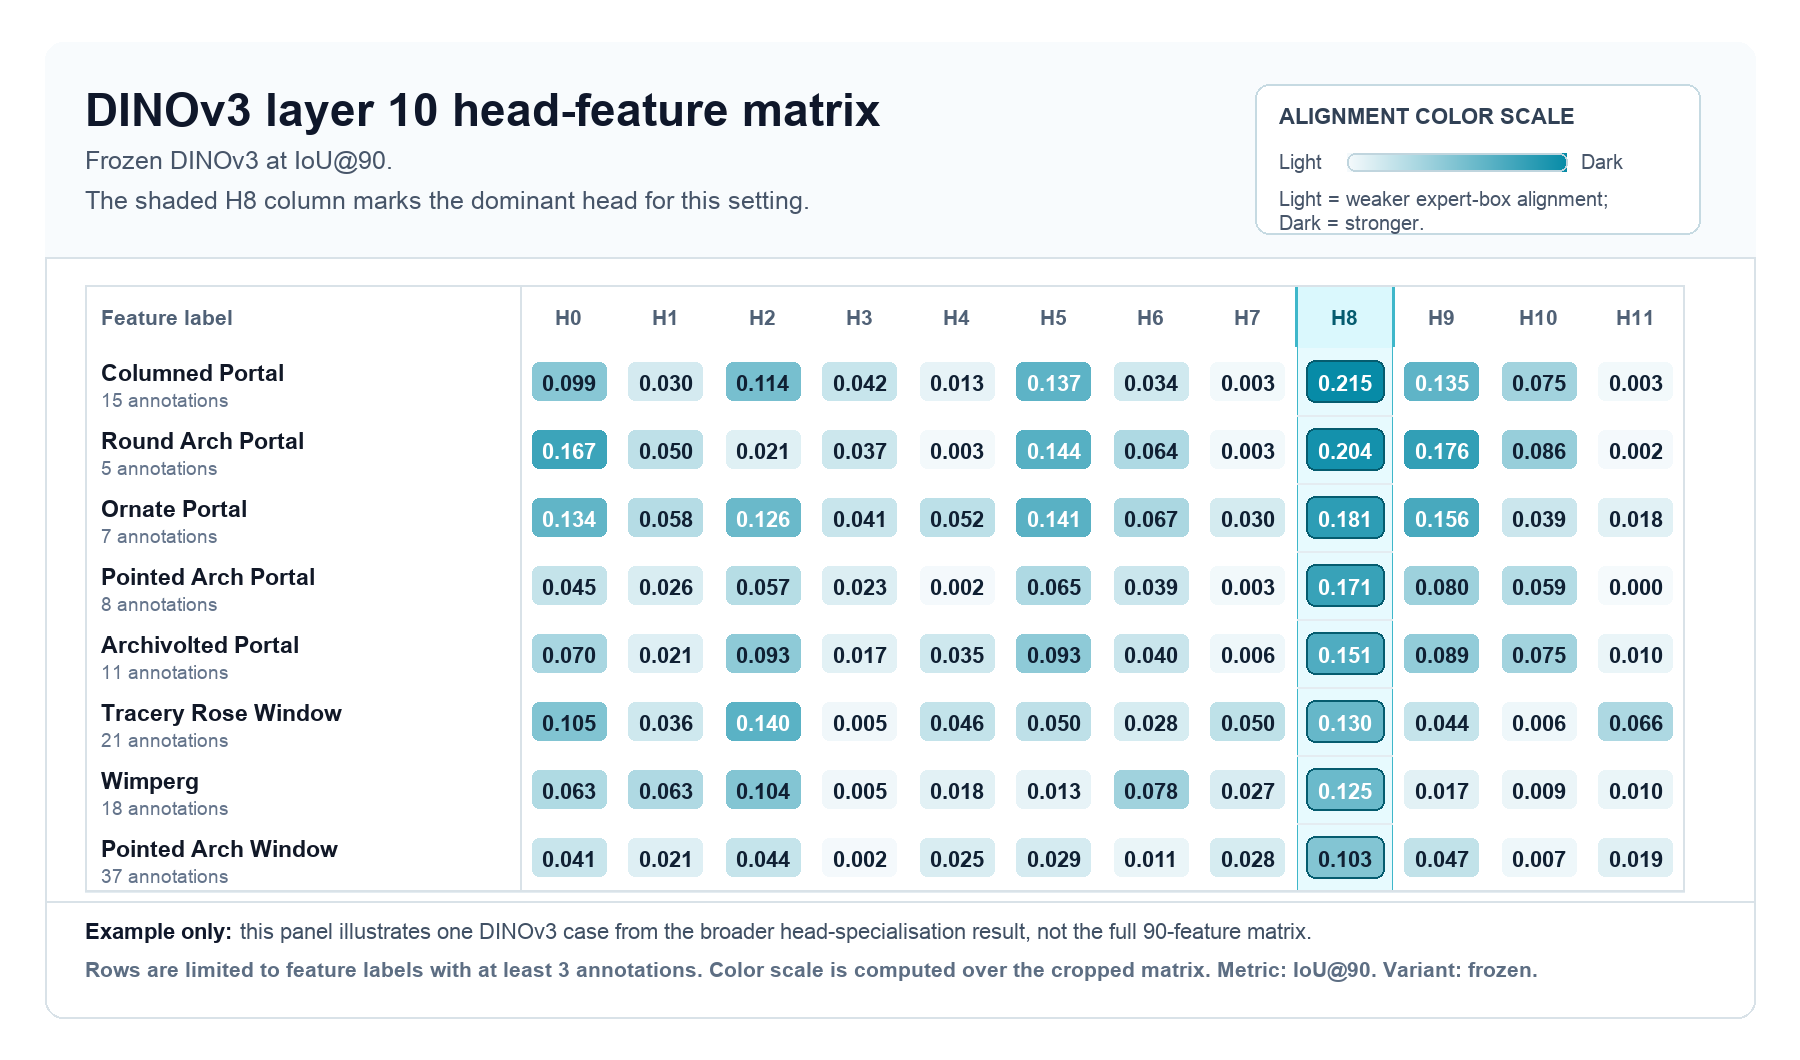
\includegraphics[width=\textwidth]{590_fig3.png}
\caption{Representative head-feature matrix for frozen DINOv3 at layer~10 using IoU@90. The shaded H8 column marks the dominant head in this setting. Lighter cells indicate weaker expert-annotated box alignment, while darker cells indicate stronger expert-annotated box alignment. The feature rows show that the dominant head aligns most strongly with portal-scale and facade-scale structures.\label{figure rq2_head_feature_matrix}}
\end{figure}

The second experiment examines the strongest and weakest feature alignments for each model's best-performing head. For each model, we identify its IoU@90 dominant head and rank all architectural features with at least three annotations. Figure~\ref{figure RQ2 top bottom} illustrates the two strongest and two weakest supported features for each model. DINOv3's \texttt{layer10/head8} reaches mean feature-level IoU@90 of 0.215 on \emph{Columned Portal}, 0.204 on \emph{Round Arch Portal}, and 0.181 on \emph{Ornate Portal}, while its weakest supported features are near zero for \emph{Blind Tracery}, \emph{Crocket}, and \emph{Tabernacle}. DINOv2's strongest supported features are \emph{Ornate Portal} and \emph{Tracery Rose Window}, and it shows a similar failure boundary on small details. MAE also favours large facade parts, although its third-strongest feature is \emph{Wimperg}. CLIP's inclusion of \emph{Belt Course} indicates that feature extent and clean geometry also influence alignment. The strongest heads obtain spatial patterns compatible with expert-annotated structural parts. The weak cases show that poorly aligned features tend to be small, thin, and repeated across model families.

\begin{figure}[!h]
\centering
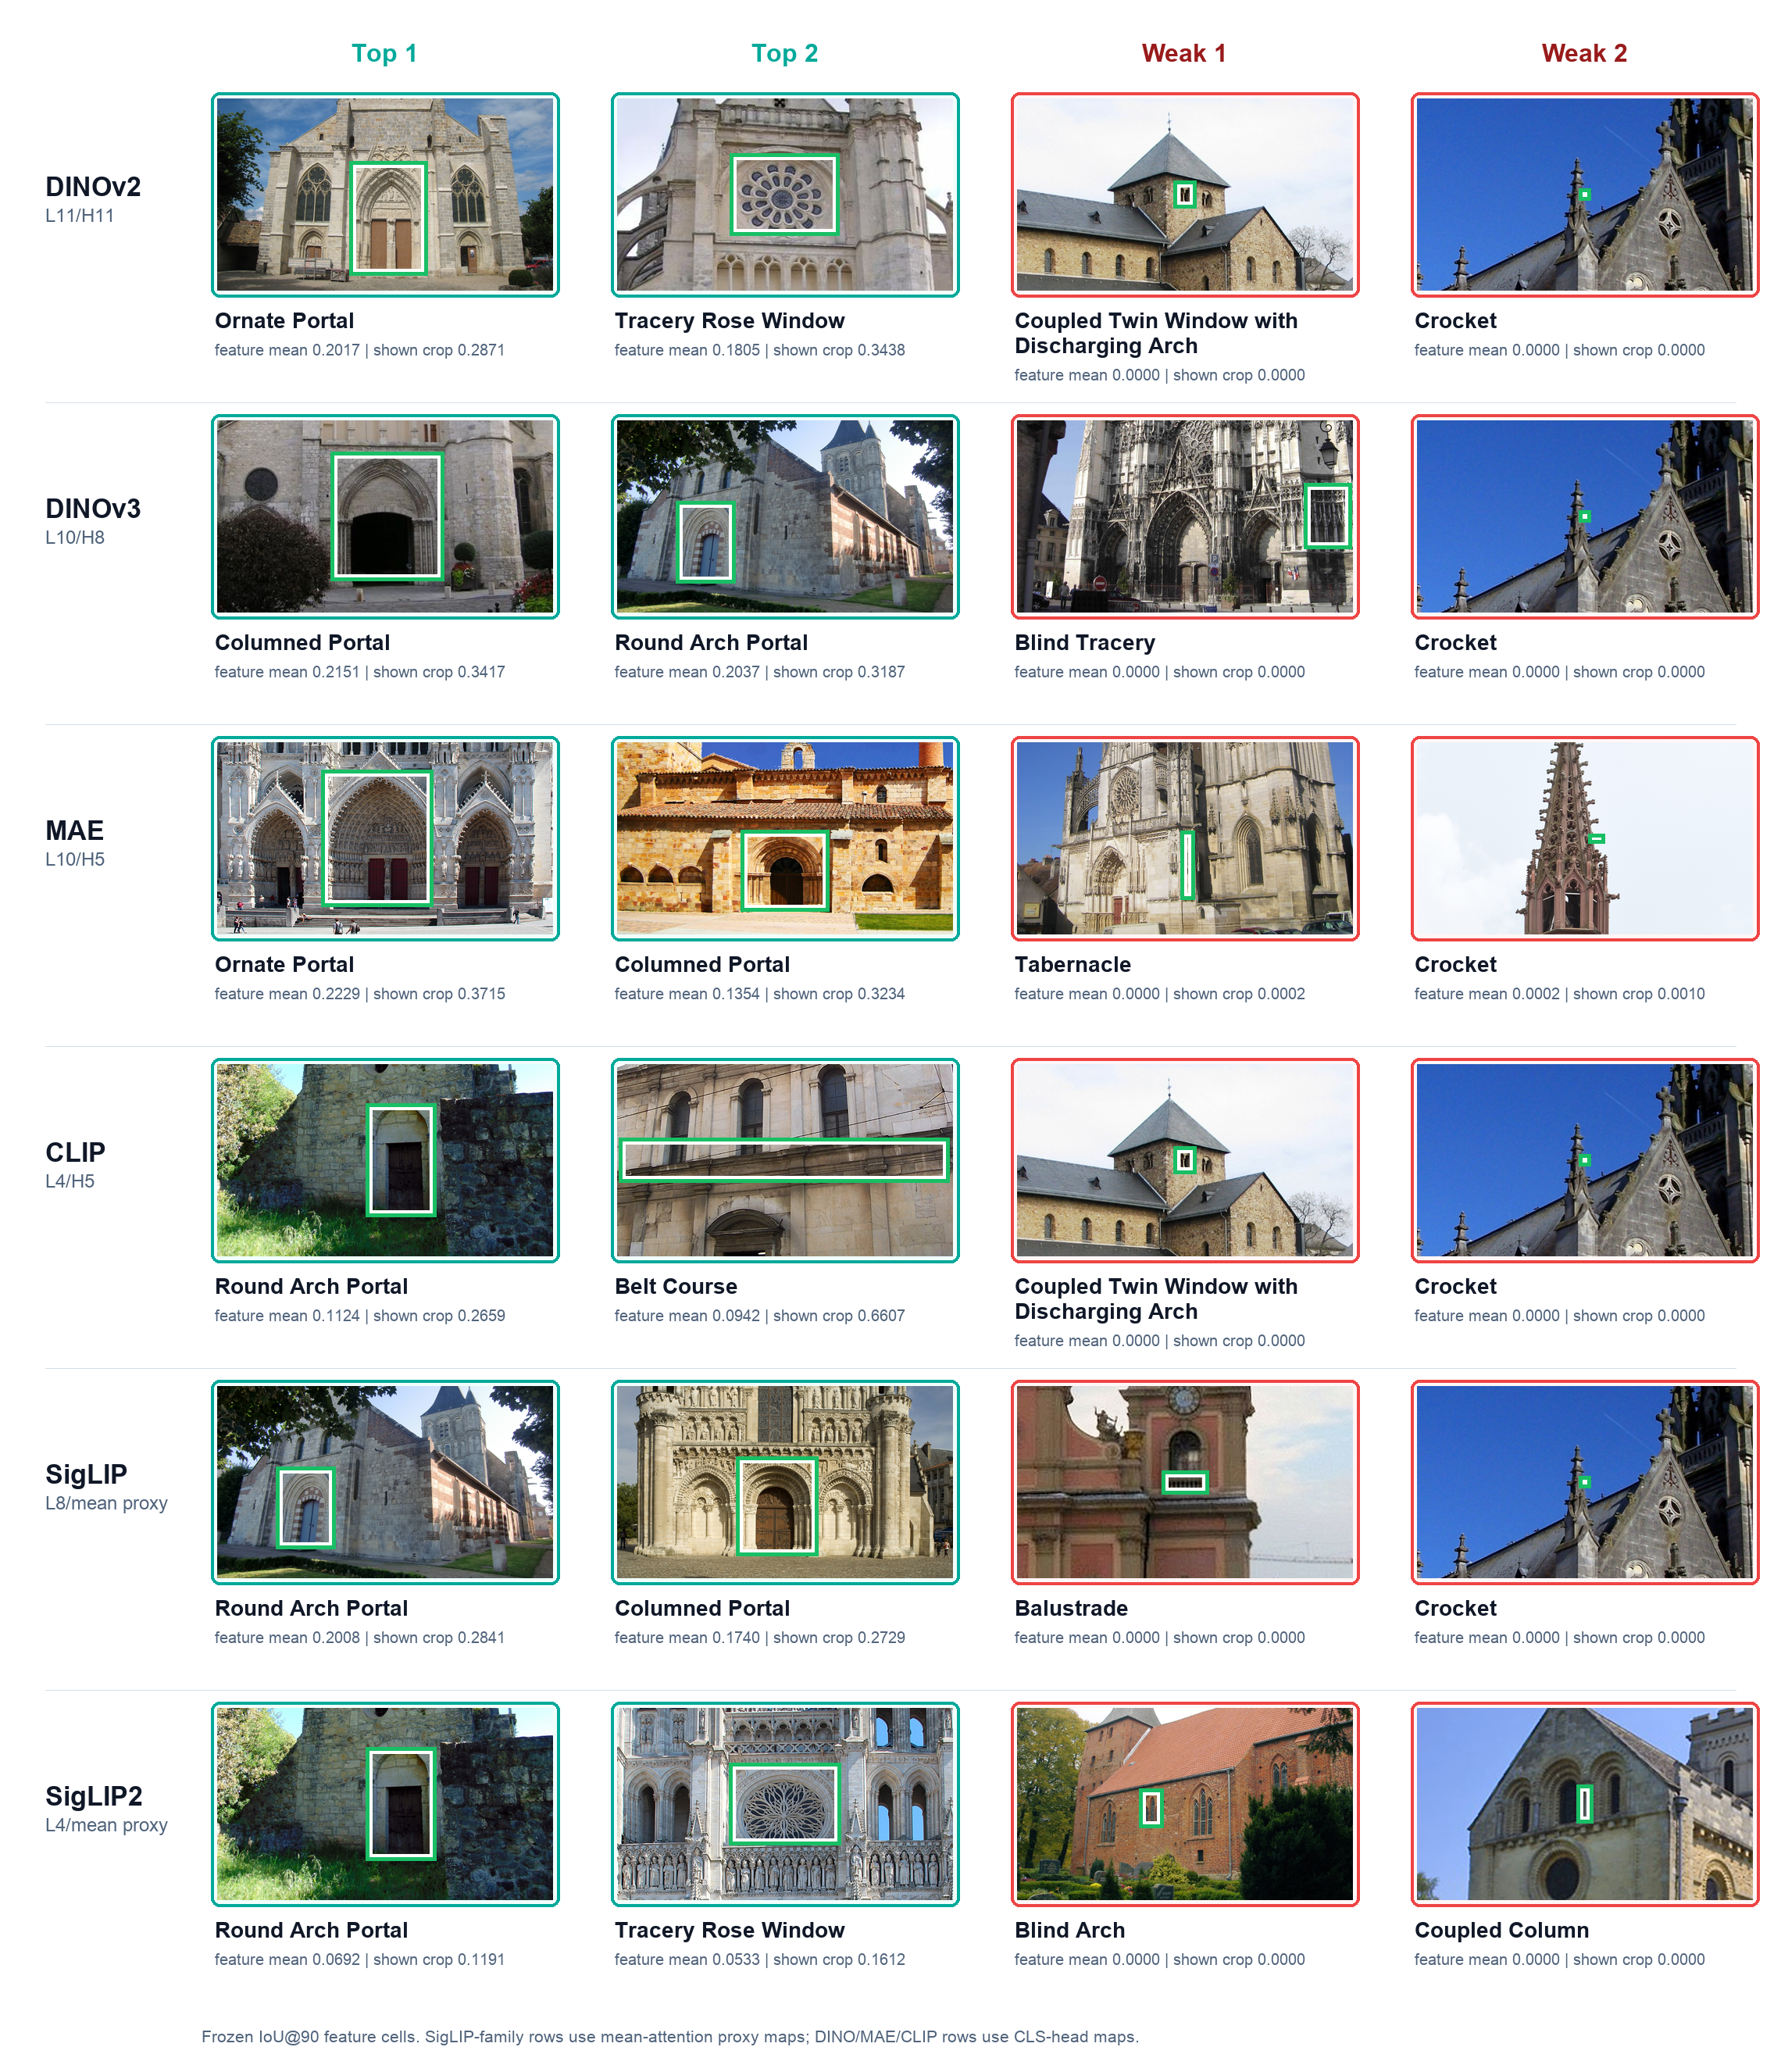
\includegraphics[width=\textwidth]{633_fig4.png}
\caption{Two strongest and two weakest feature alignments for each model's dominant frozen head. DINOv2 \texttt{layer11/head11}, DINOv3 \texttt{layer10/head8}, MAE \texttt{layer10/head5}, CLIP \texttt{layer4/head5}, SigLIP \texttt{layer8/mean proxy}, and SigLIP2 \texttt{layer4/mean proxy}. Green panels indicate high-alignment feature cells, and red panels indicate weak feature cells.\label{figure RQ2 top bottom}}
\end{figure}

\clearpage

\subsection{Results from RQ3: The effect of downstream adaptation}

The RQ3 examines how downstream adaptation changes attention alignment with expert-annotated architectural regions. We compare three adaptation strategies: linear probing, LoRA, and full fine-tuning. Figure~\ref{figure RQ3 heatmap} summarizes the mean change relative to the frozen model across all models, metrics, and adaptation strategies. Figure~\ref{figure RQ3 forest} complements this summary with 95\% bootstrap confidence intervals, providing a statistical view of the same changes. Table~\ref{table RQ3 perstyle} further decomposes the full fine-tuning results by architectural style, reporting per-style changes in IoU@90.

\begin{figure}[!ht]
\centering
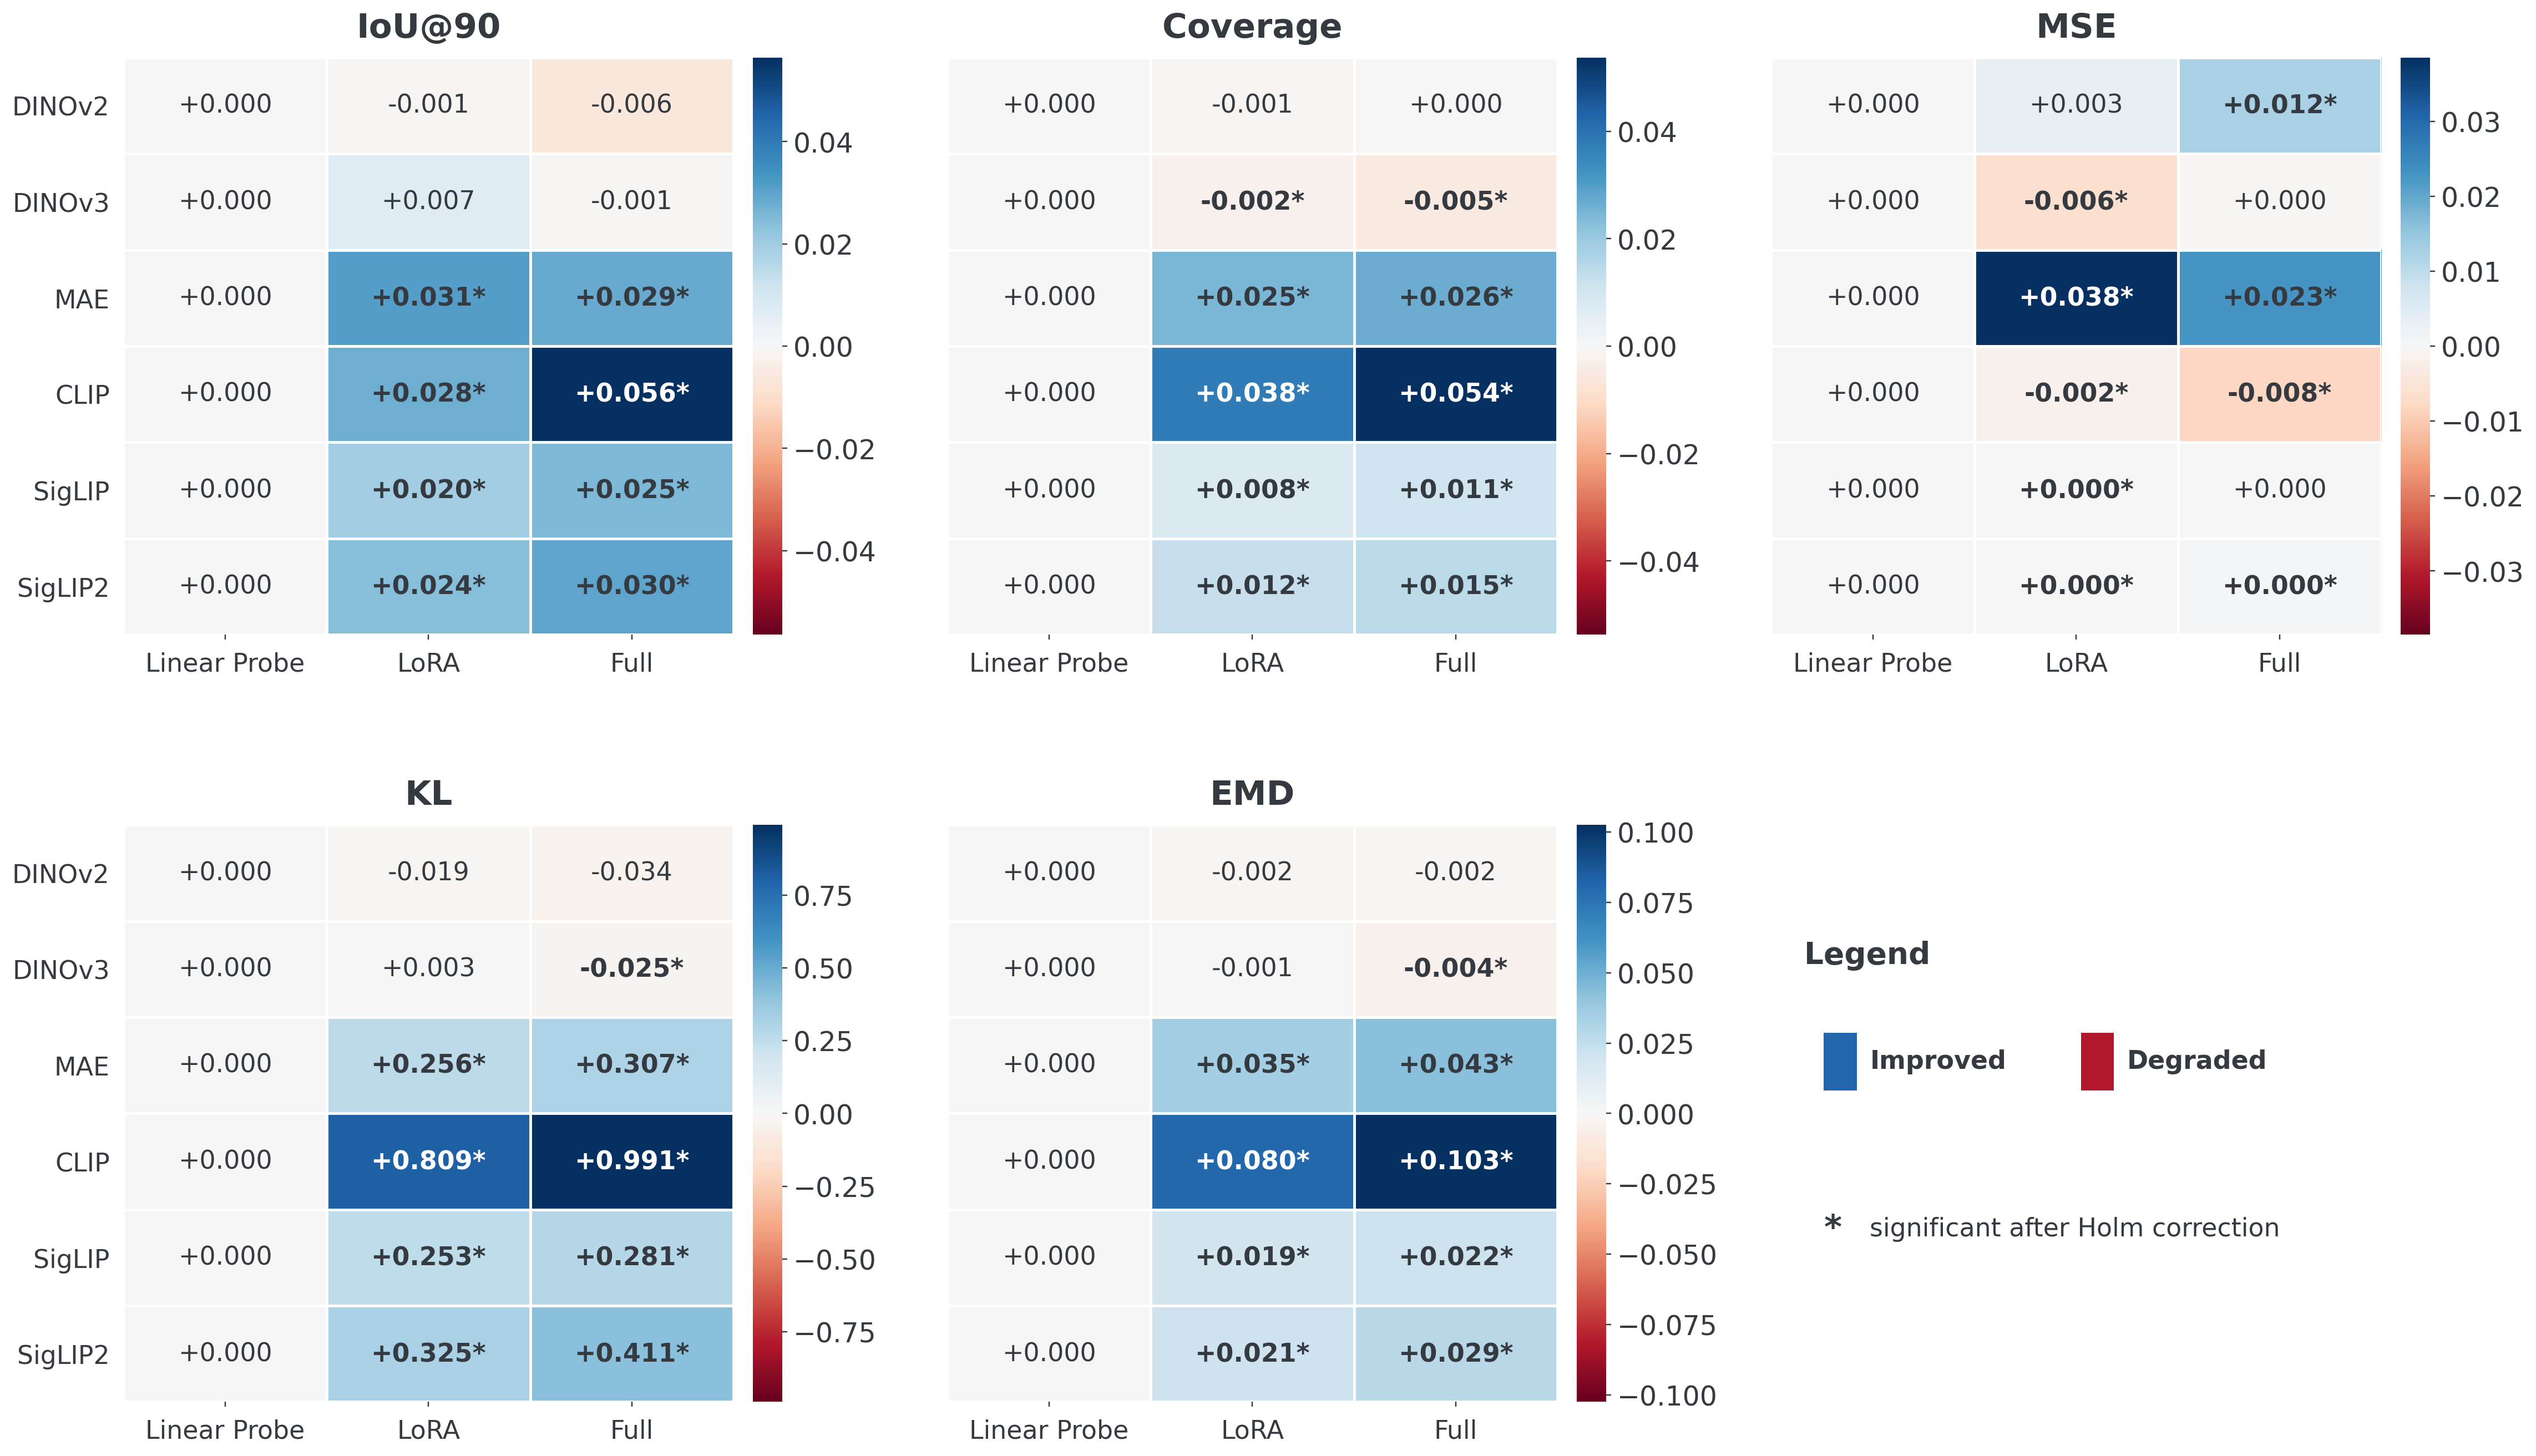
\includegraphics[width=\textwidth]{667_fig5.png}
\caption{Attention-alignment changes under downstream adaptation. Each cell reports the mean change relative to the frozen model for the linear probe, LoRA, and full fine-tuning across DINOv2, DINOv3, MAE, CLIP, SigLIP, and SigLIP2. Blue cells indicate improvement in the corresponding metric and red cells indicate degradation; asterisks mark effects that remain significant after Holm correction. \label{figure RQ3 heatmap}}
\end{figure}

\begin{figure}[!ht]
\centering
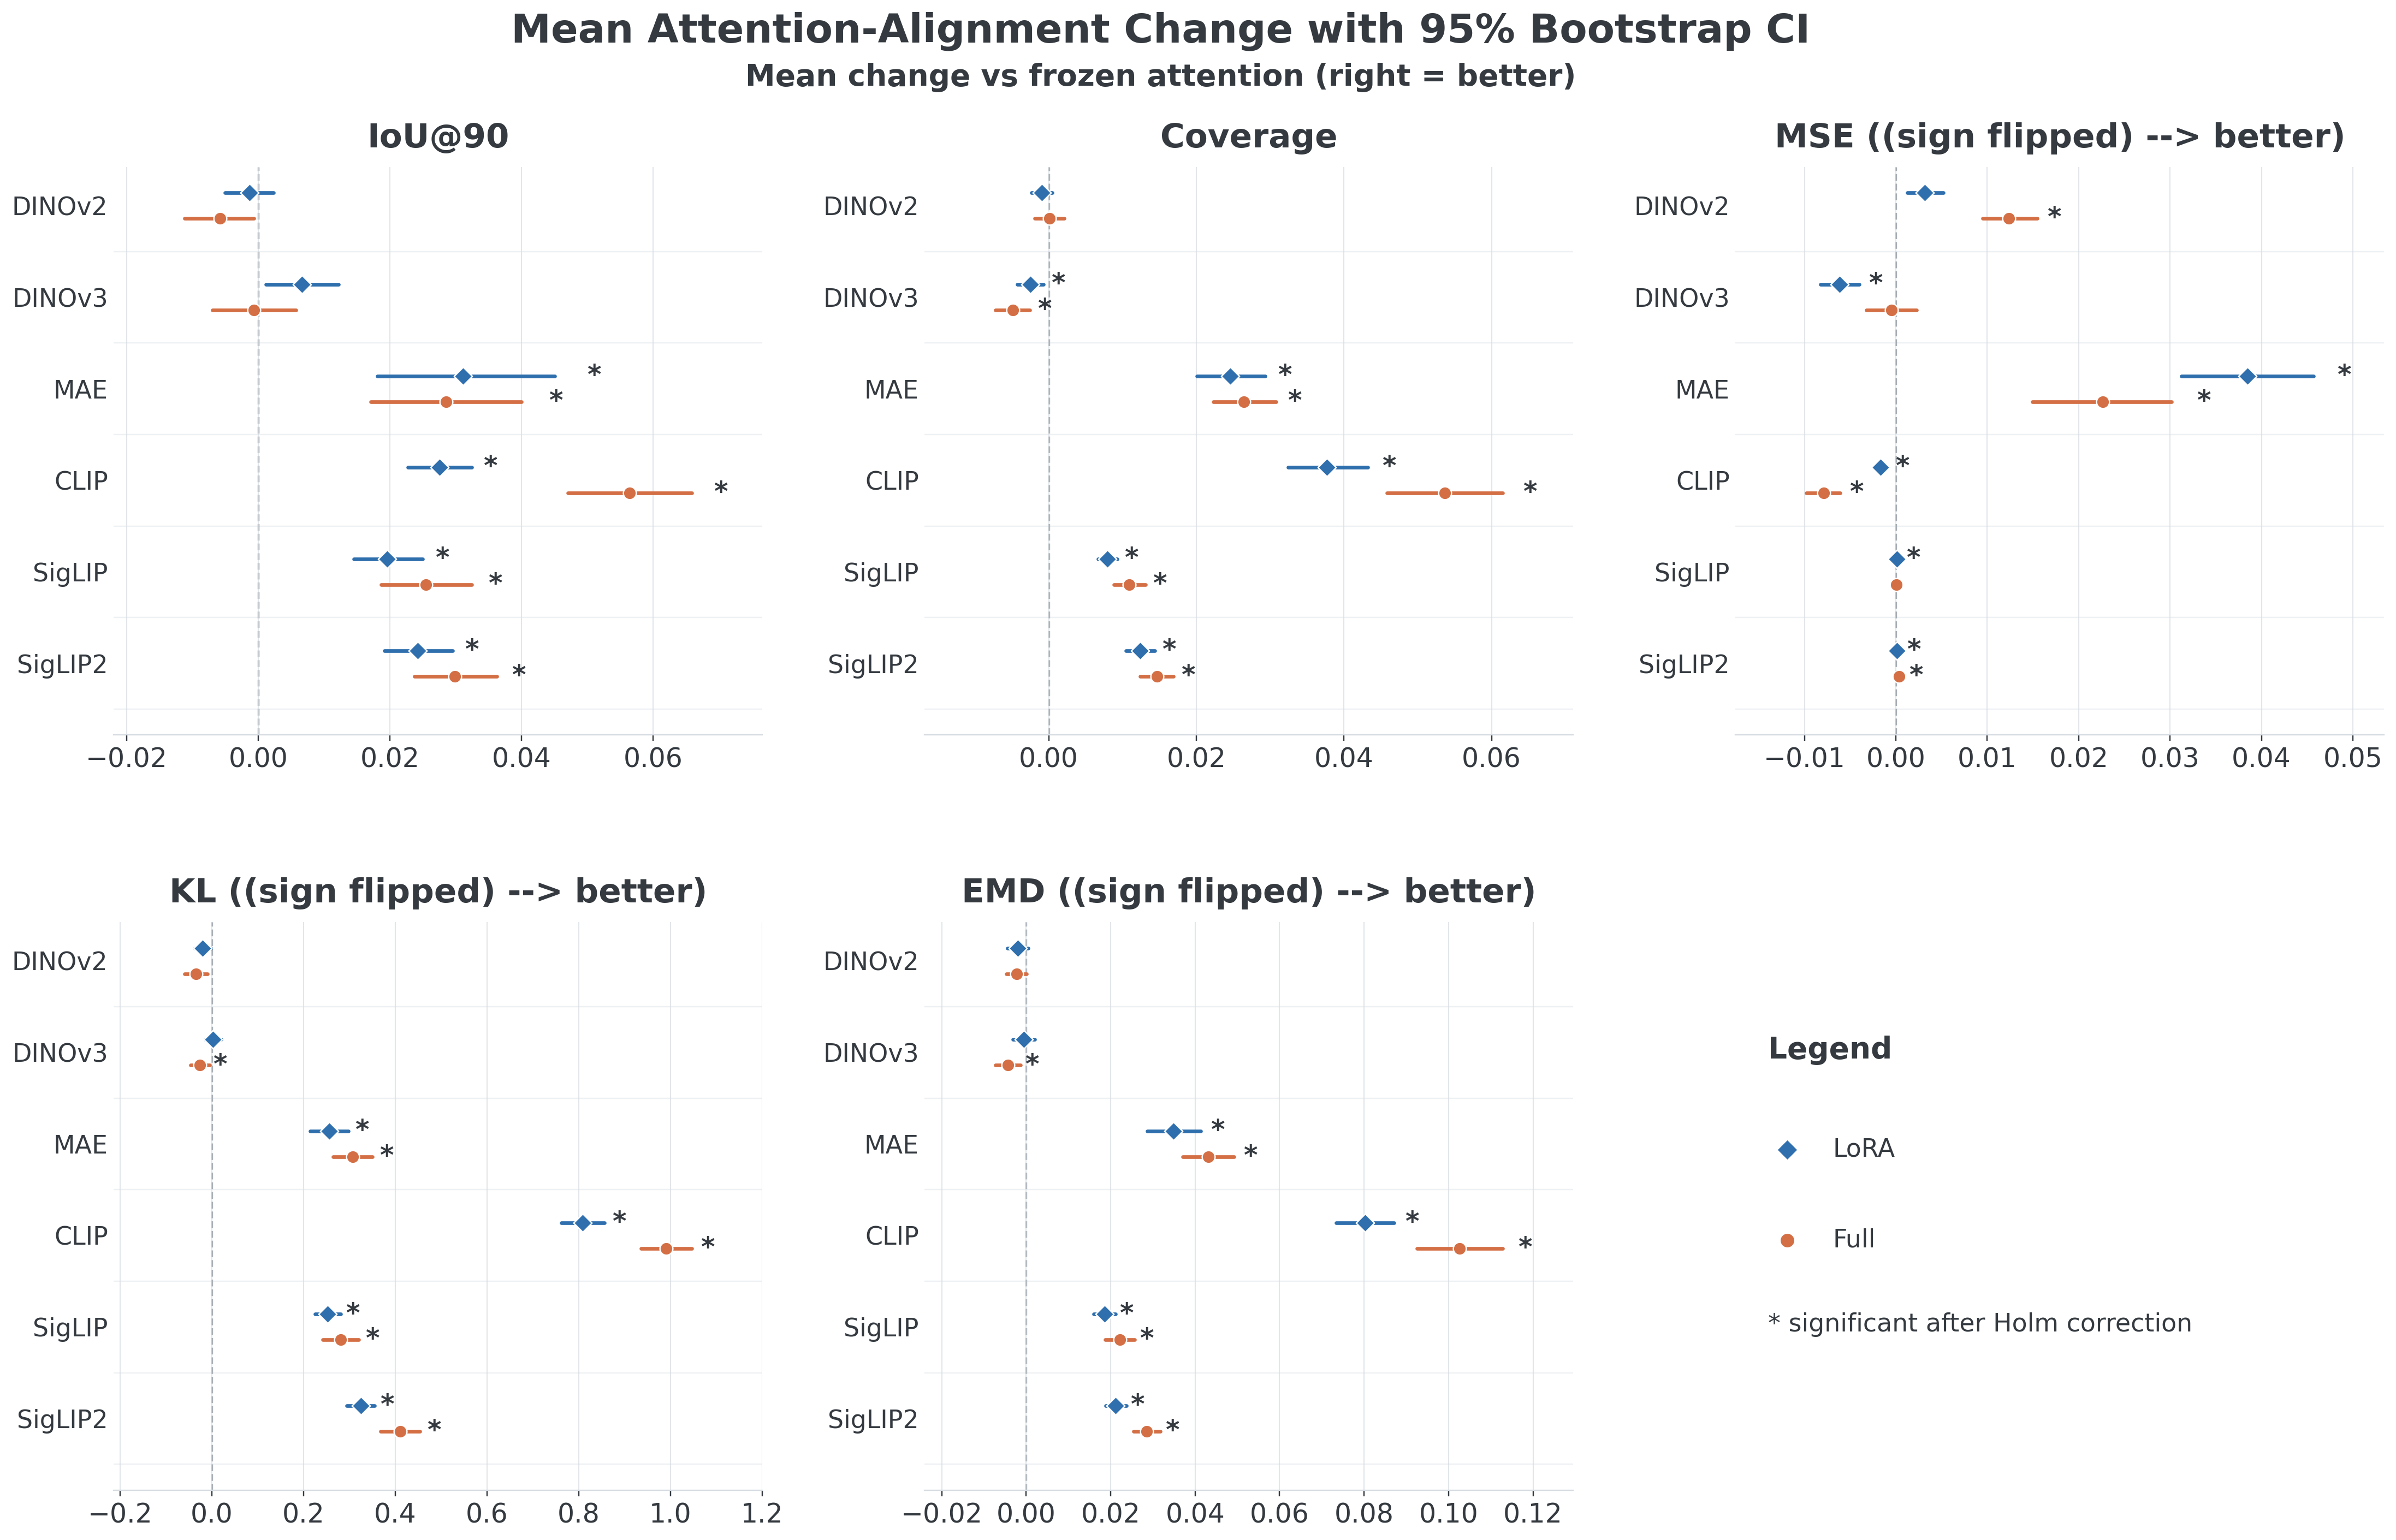
\includegraphics[width=\textwidth]{714_fig6.png}
\caption{Mean attention-alignment change with 95\% bootstrap confidence intervals. Each figure reports the change relative to the frozen model for LoRA and full fine-tuning. For MSE, KL divergence, and EMD, signs are flipped so that rightward movement consistently indicates improvement. Asterisks mark effects that remain significant after Holm correction.\label{figure RQ3 forest}}
\end{figure}

\begin{table}[!h]
\centering
\caption{Per-style $\Delta$IoU@90 under full fine-tuning. Positive values indicate improved attention alignment relative to frozen attention.}
\label{table RQ3 perstyle}
\begin{tabular}{lcccc}
\toprule
Vision foundation model & Romanesque & Gothic & Renaissance & Baroque \\ \midrule
DINOv2  & $-$0.001 & +0.010 & $-$0.006 & $-$0.007 \\
DINOv3  & $-$0.003 & +0.006 & $-$0.004 & $-$0.009 \\
MAE     & +0.007 & +0.009 & +0.108 & +0.045 \\
CLIP    & +0.084 & +0.091 & +0.020 & +0.017 \\
SigLIP  & +0.033 & +0.039 & $-$0.006 & +0.005 \\
SigLIP2 & +0.034 & +0.044 & +0.007 & +0.007 \\
\bottomrule
\end{tabular}
\end{table}

The effect of adaptation differs across model families. DINOv2 and DINOv3 show small $\Delta$ values across styles and adaptation strategies. Their aggregate $\Delta$IoU@90 ranges from $-$0.001 to +0.009 under LoRA and full fine-tuning, and their per-style values under full fine-tuning stay within $\pm$0.010. The only significant aggregate IoU@90 change among them is a modest LoRA gain for DINOv2 (+0.009). This can be explained because expert-aligned spatial structure is already present in the pretrained representations, and the style-classification objective is absorbed by the classification head rather than reshaping backbone attention. CLIP shows the largest overall improvement after full fine-tuning. Its IoU@90 increases from 0.0229 to 0.0910, and its Coverage increases from 0.054 to 0.121, with a Cohen's $d \approx 1.05$. The style-level breakdown shows that this gain is concentrated mainly in Romanesque (+0.084) and Gothic (+0.091) images. In contrast, Renaissance (+0.020) and Baroque (+0.017) show much smaller gains. MAE shows a different adaptation profile. Its largest shift occurs for Renaissance images, where full fine-tuning produces a $\Delta$IoU@90 of +0.108. The SigLIP-family models show moderate but interpretable gains. Under full fine-tuning, SigLIP remains higher in absolute IoU@90, whereas SigLIP2 moves further in standardized-effect terms. 

The per-style results indicate that adaptation effects are not uniform across architectural categories. A Kruskal-Wallis test finds significant style moderation for CLIP ($p=7.6\times10^{-9}$), MAE ($p=3.9\times10^{-7}$), SigLIP ($p=4.4\times10^{-6}$), and SigLIP2 ($p=6.6\times10^{-7}$); DINOv2 and DINOv3 do not show significant style moderation ($p=0.22$, $p=0.11$), consistent with their small per-style change profiles. These results suggest that adaptation mainly reshapes attention for models whose frozen spatial alignment is initially weaker or more style-dependent.

We further examine whether adaptation changes the dominant layer and attention head responsible for expert alignment. Figure~\ref{figure RQ3 head ranking} reports the top three layer-head locations for each model and adaptation strategy, ranked by mean IoU@90. DINOv3 provides the clearest case of head stability: the same \texttt{layer10/head8} remains the best-aligned head across frozen, LoRA, and full fine-tuning. DINOv2 shows the same preserved-head pattern: \texttt{layer11/head11} remains its best-aligned head across frozen, LoRA, and full fine-tuning, at a similar absolute level to DINOv3. MAE is more flexible: its dominant head shifts from \texttt{layer10/head5} in the frozen model to \texttt{layer11/head7} under LoRA, and then returns to \texttt{layer10/head5} under full fine-tuning. CLIP shows the strongest reorganization. In the frozen model, its best heads are located in early layers, with \texttt{layer4/head5} leading. After adaptation, however, a late-layer head in \texttt{layer11} becomes the strongest adapted location, while \texttt{layer4/head5} remains close to its frozen score. Thus, CLIP's late-layer alignment is newly strengthened by adaptation rather than inherited from an already strong frozen late-layer head.

\begin{figure}[!h]
\centering
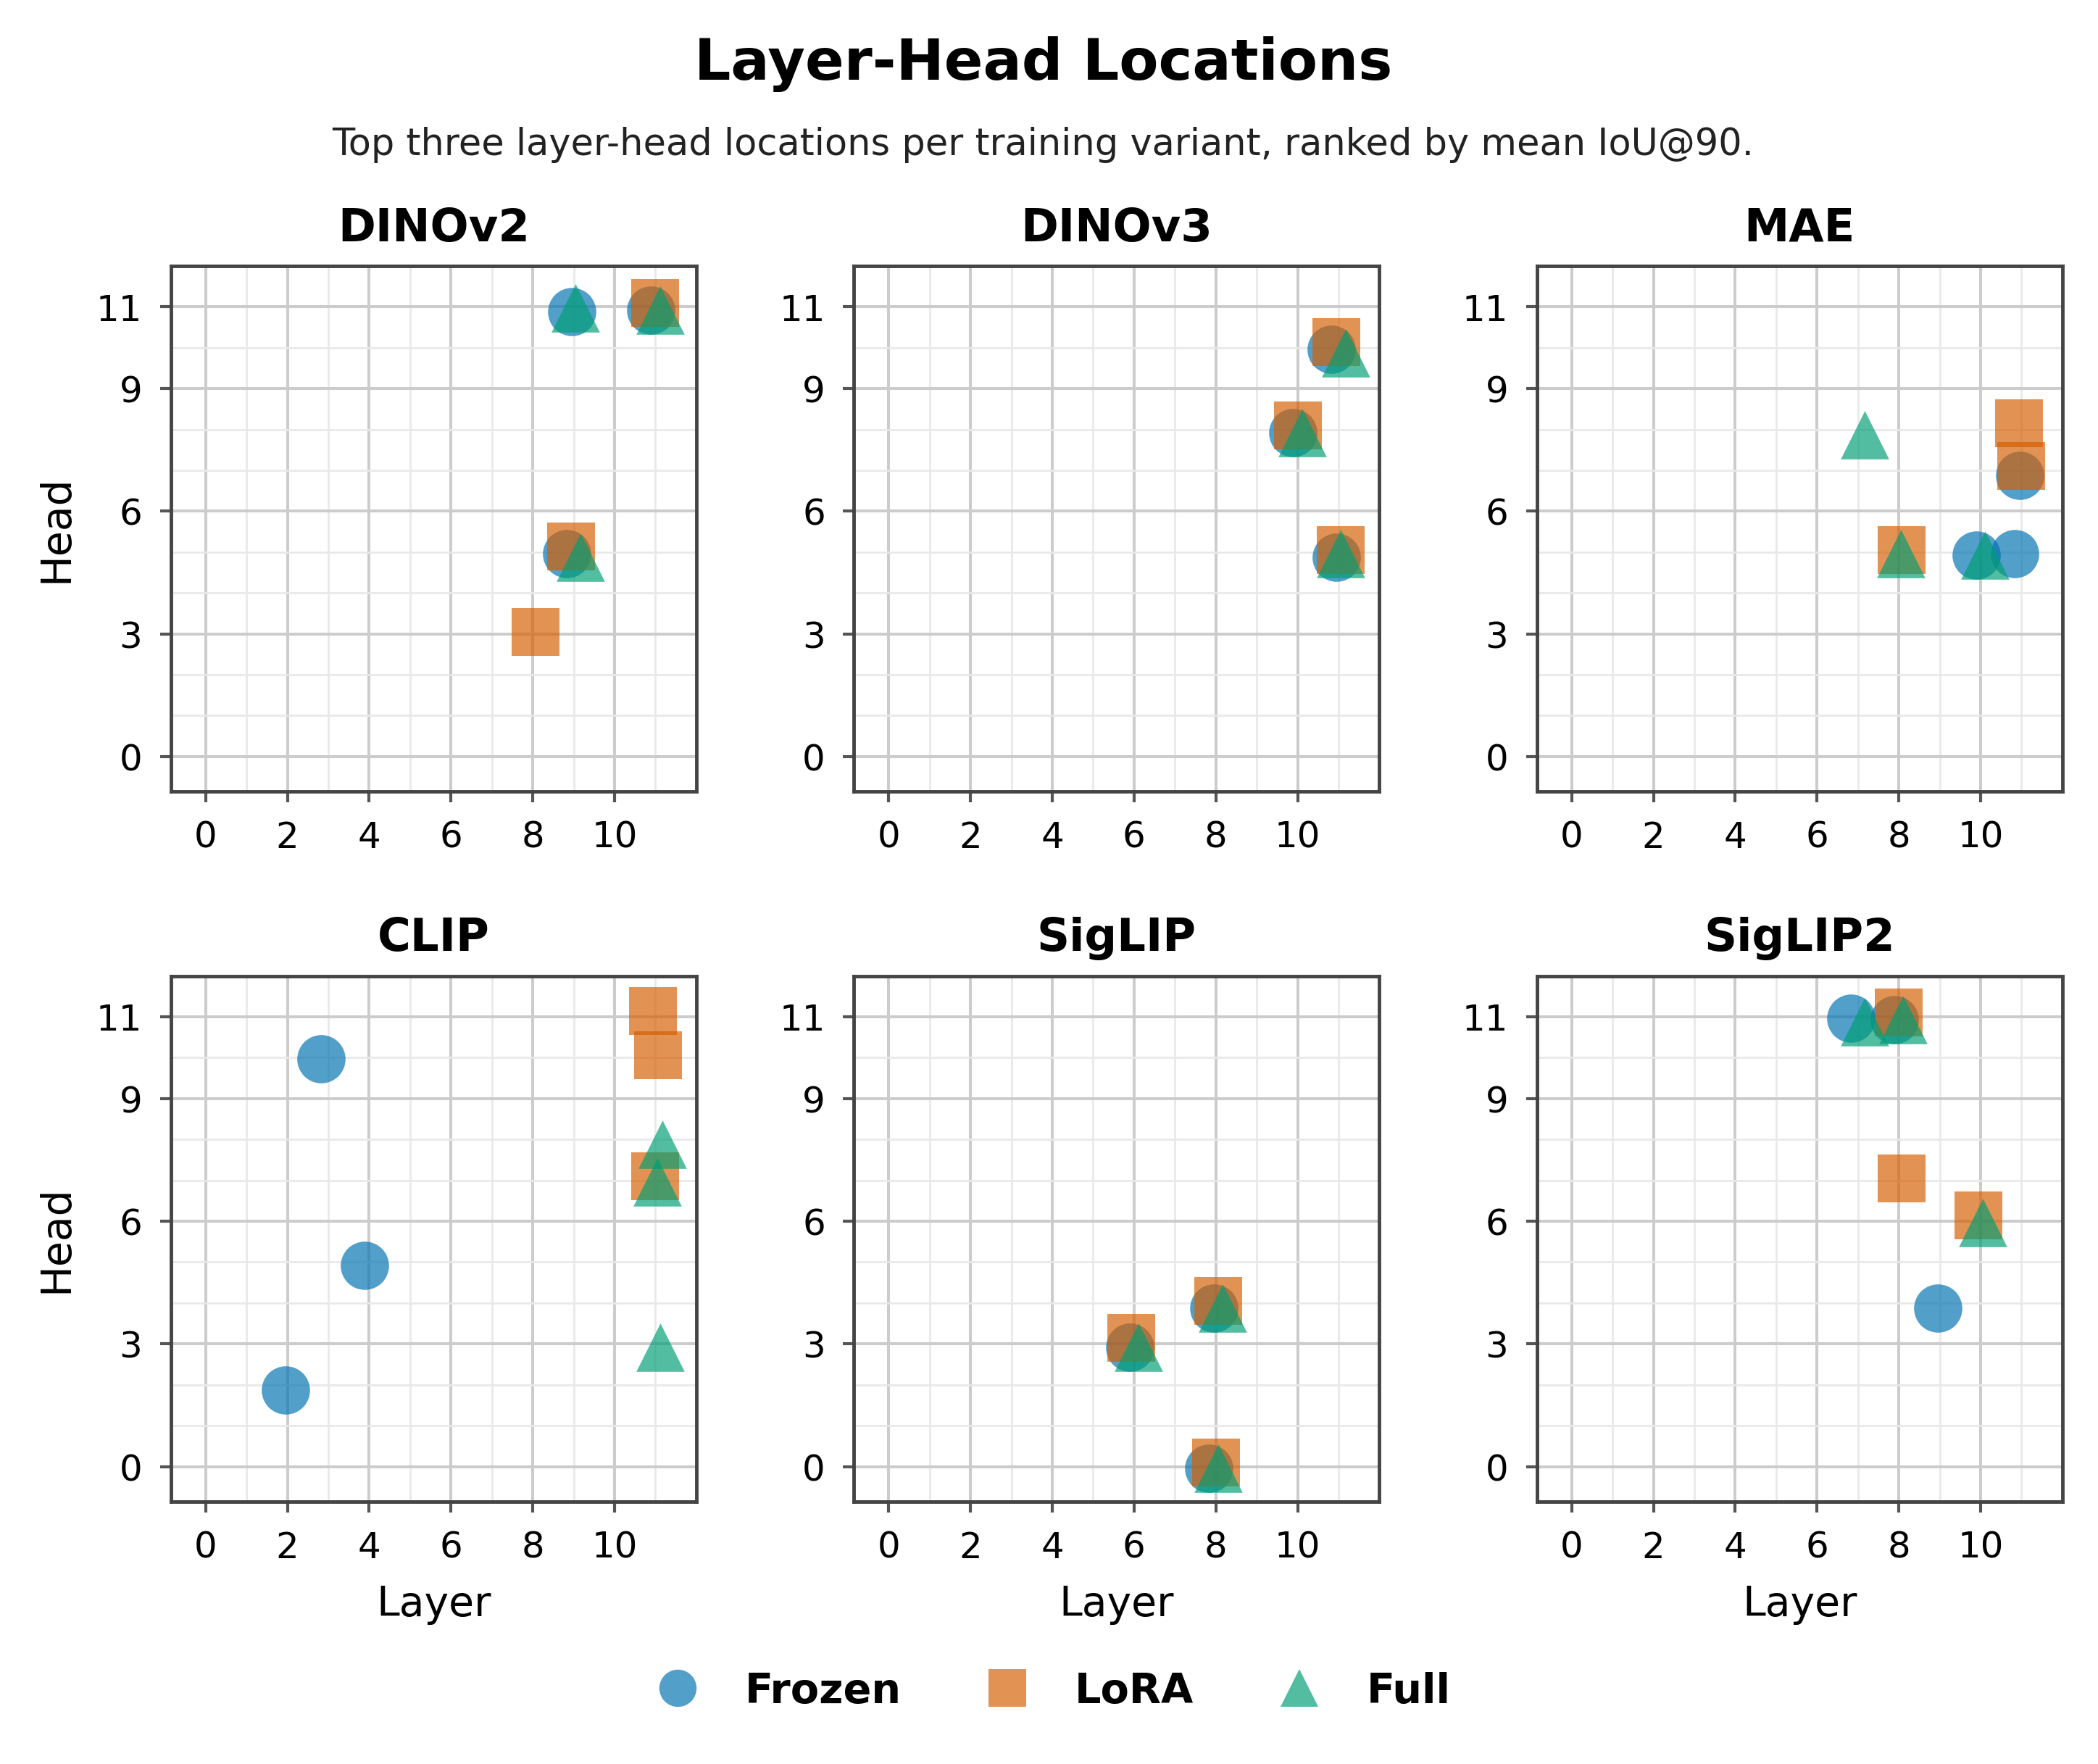
\includegraphics[width=\textwidth]{787_tbl7_enlarge.png}
\caption{Dominant layer-head locations under different adaptation strategies. Each figure shows the top three layer-head locations ranked by mean IoU@90. The linear probe is omitted because it freezes the backbone and therefore does not create a new attention-head configuration.\label{figure RQ3 head ranking}}
\end{figure}

\subsubsection{Relation to classification correctness}\label{section RQ3 correctness}

Attention alignment does not replace classification accuracy as an evaluation criterion, so we also related each run's classification correctness to its attention alignment on the 139 expert-annotated images. Figure~\ref{figure RQ3 accuracy alignment} plots each run's accuracy against its mean IoU@90 at layer 11. Table~\ref{table RQ3 correctness} compares the per-image IoU@90 of correctly and wrongly classified images within each run, using a two-sided Mann-Whitney U test with Holm adjustment across the 18 runs. Accuracy and alignment do not rank the models in the same order. DINOv2 and DINOv3 combine the highest alignment with accuracies from 0.856 to 0.906, whereas CLIP, SigLIP, and SigLIP2 reach accuracies from 0.820 to 0.899 with a mean IoU@90 of at most 0.091. Frozen MAE has the lowest accuracy (0.518). Adaptation increased accuracy in 11 of the 12 adapted runs; the exception is DINOv2 under full fine-tuning (0.871 to 0.856).

\begin{figure}[!htbp]
\centering
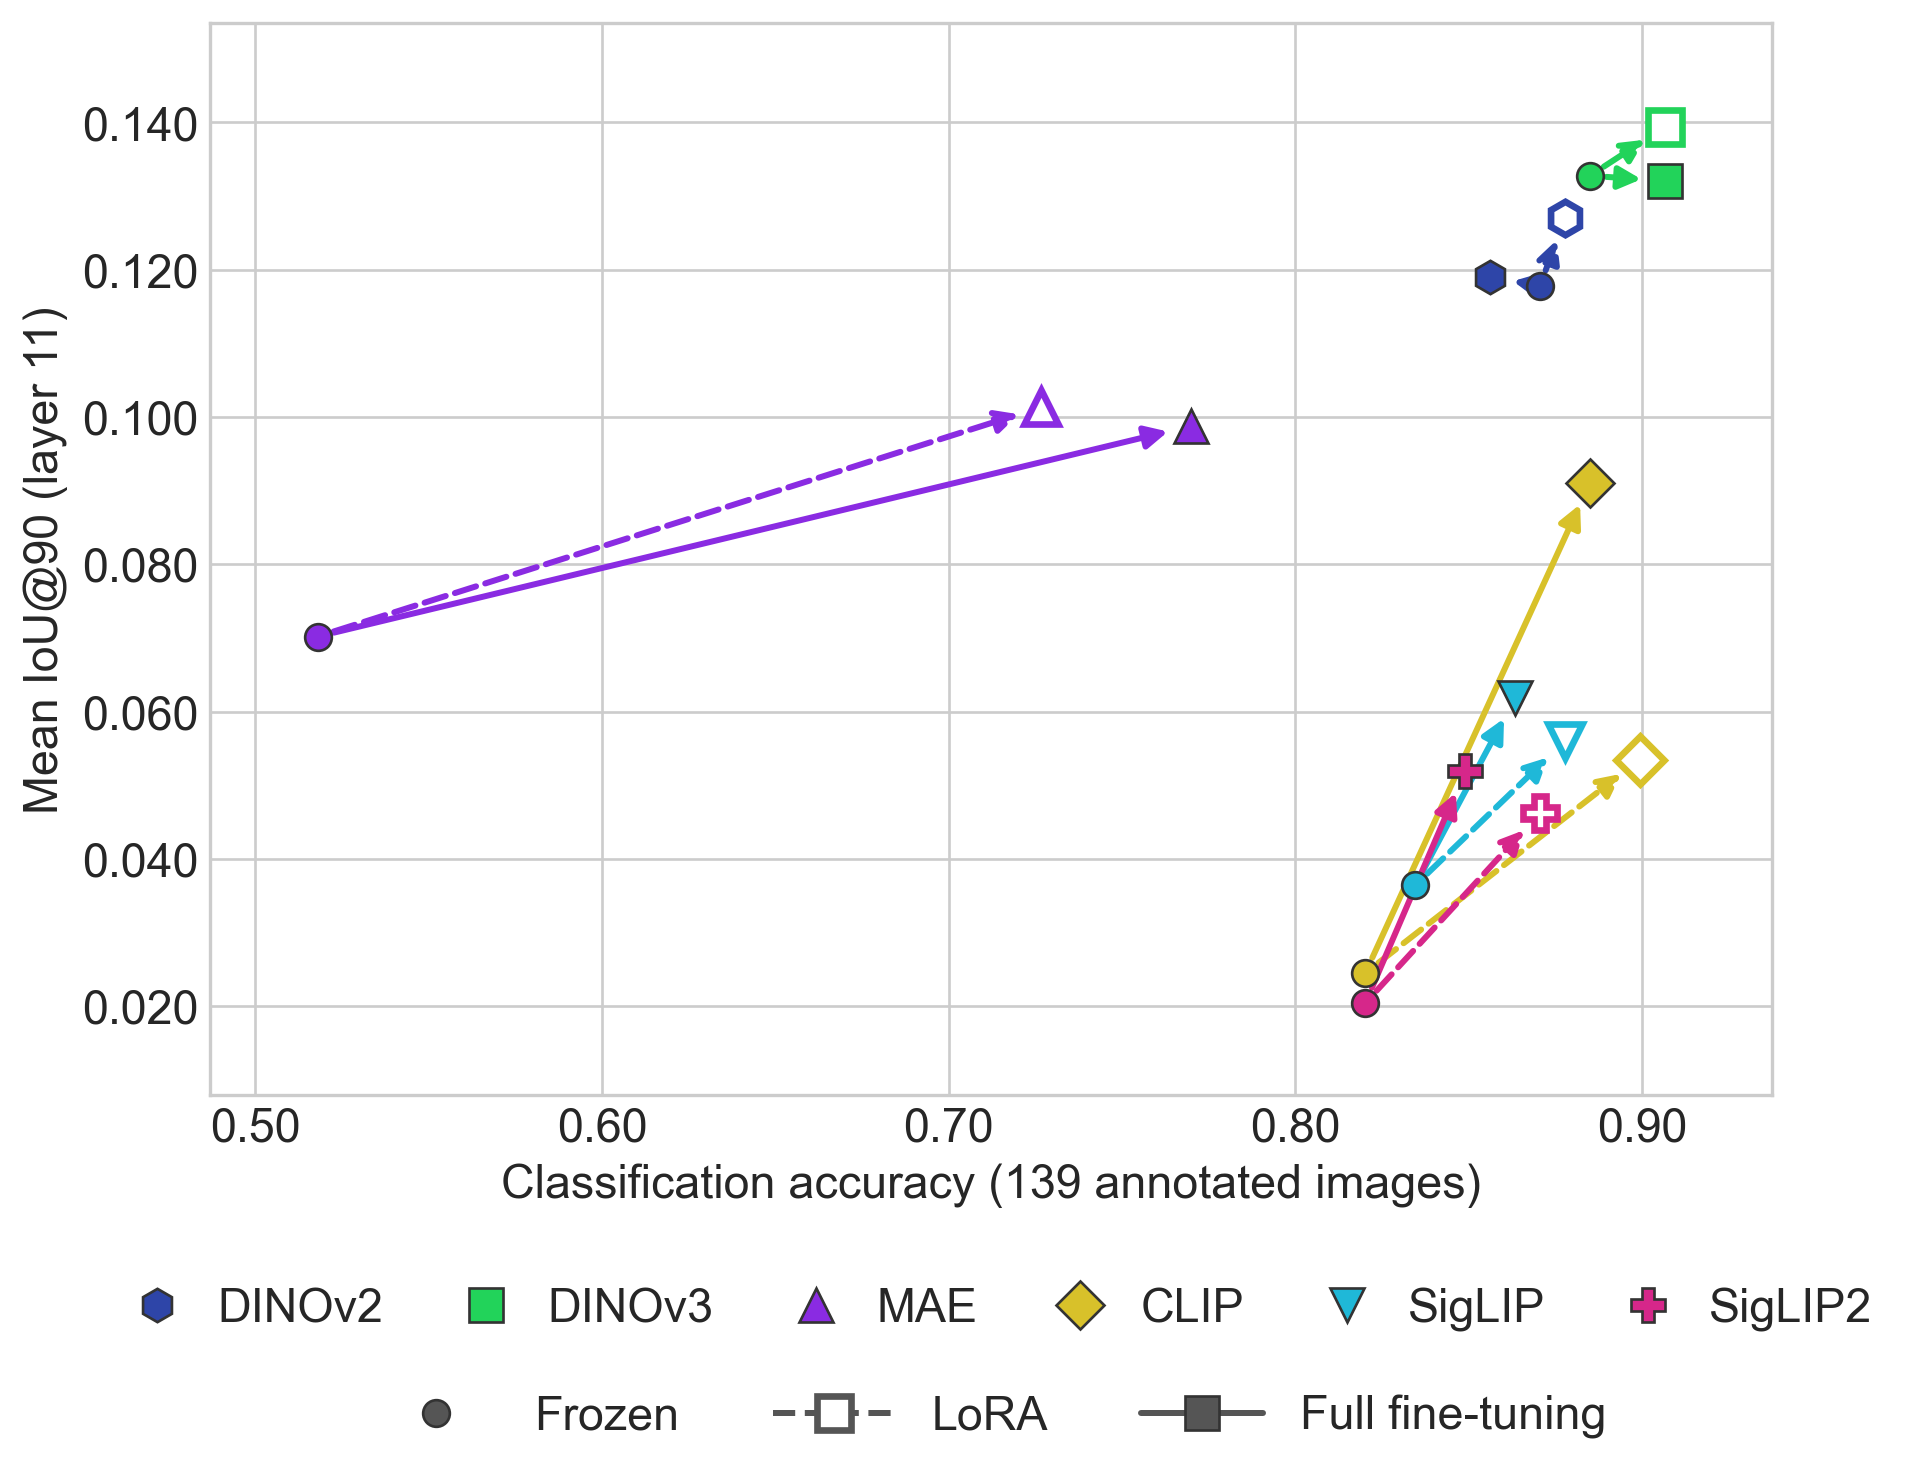
\includegraphics[width=0.85\textwidth]{RQ3_accuracy_alignment.png}
\caption{Classification accuracy and attention alignment on the 139 expert-annotated images. Each point is one run, with accuracy on the horizontal axis and mean IoU@90 at layer 11 on the vertical axis. Color identifies the model. Circles show the frozen backbone with its trained linear classifier. Hollow and filled model markers show the LoRA and fully fine-tuned checkpoints, and dashed and solid arrows lead to them from the frozen model. Frozen CLIP and SigLIP2 have the same accuracy (0.820) and nearly the same mean IoU@90 (0.023 and 0.022), so their circles are offset vertically by 0.0016 to keep both visible.\label{figure RQ3 accuracy alignment}}
\end{figure}

\begin{table}[!htbp]
\centering
\caption{Classification correctness and attention alignment on the 139 expert-annotated images. Accuracy and balanced accuracy use the expert-annotation style labels. Median IoU@90 at layer 11 is reported separately for correctly and wrongly classified images. $p_{\text{Holm}}$ is the two-sided Mann-Whitney U $p$-value comparing the two groups, Holm-adjusted across the 18 runs. Bold marks $p_{\text{Holm}} < 0.05$.\label{table RQ3 correctness}}
\begin{tabular}{llccrrccc}
\toprule
 & & & & \multicolumn{2}{c}{Images} & \multicolumn{2}{c}{Median IoU@90} & \\
Model & Strategy & Acc. & Bal. acc. & Correct & Wrong & Correct & Wrong & $p_{\text{Holm}}$ \\ \midrule
DINOv2   & Frozen & 0.871 & 0.840 & 121 & 18 & 0.1039 & 0.0535 & 0.661 \\
         & LoRA   & 0.878 & 0.845 & 122 & 17 & 0.1145 & 0.0675 & 0.661 \\
         & Full   & 0.856 & 0.795 & 119 & 20 & 0.1276 & 0.0608 & 0.231 \\ \midrule
DINOv3   & Frozen & 0.885 & 0.847 & 123 & 16 & 0.1085 & 0.0817 & 1.000 \\
         & LoRA   & 0.906 & 0.855 & 126 & 13 & 0.1263 & 0.0479 & 0.076 \\
         & Full   & 0.906 & 0.855 & 126 & 13 & 0.1229 & 0.0563 & 0.213 \\ \midrule
MAE      & Frozen & 0.518 & 0.585 & 72 & 67 & 0.0362 & 0.0752 & \textbf{0.021} \\
         & LoRA   & 0.727 & 0.767 & 101 & 38 & 0.0760 & 0.0966 & 1.000 \\
         & Full   & 0.770 & 0.790 & 107 & 32 & 0.0807 & 0.0882 & 1.000 \\ \midrule
CLIP     & Frozen & 0.820 & 0.832 & 114 & 25 & 0.0083 & 0.0068 & 1.000 \\
         & LoRA   & 0.899 & 0.870 & 125 & 14 & 0.0445 & 0.0363 & 1.000 \\
         & Full   & 0.885 & 0.834 & 123 & 16 & 0.0779 & 0.0434 & 0.226 \\ \midrule
SigLIP   & Frozen & 0.835 & 0.845 & 116 & 23 & 0.0230 & 0.0090 & 0.231 \\
         & LoRA   & 0.878 & 0.836 & 122 & 17 & 0.0429 & 0.0091 & \textbf{0.031} \\
         & Full   & 0.863 & 0.803 & 120 & 19 & 0.0457 & 0.0128 & \textbf{0.041} \\ \midrule
SigLIP2  & Frozen & 0.820 & 0.841 & 114 & 25 & 0.0154 & 0.0097 & 1.000 \\
         & LoRA   & 0.871 & 0.869 & 121 & 18 & 0.0391 & 0.0231 & 0.231 \\
         & Full   & 0.849 & 0.809 & 118 & 21 & 0.0425 & 0.0301 & 1.000 \\
\bottomrule
\end{tabular}
\end{table}

Within runs, correctly classified images had a higher median IoU@90 than misclassified images in 15 of the 18 runs. The exceptions are the three MAE runs. After Holm correction, the difference is significant in only three runs. For SigLIP under LoRA ($p_{\text{Holm}}=0.031$) and full fine-tuning ($p_{\text{Holm}}=0.041$), correctly classified images aligned better. For frozen MAE ($p_{\text{Holm}}=0.021$), misclassified images aligned better. Coverage, MSE, KL divergence, and EMD show no significant difference in any run (Table~\ref{table appendix correctness}). In this benchmark, therefore, correct predictions tend to coincide with better-aligned attention, but the association is significant only for adapted SigLIP and is reversed for MAE. Most runs misclassify few images, so these tests have limited power, and a non-significant result does not show that no association exists. The comparison is also observational. It is not adjusted for style or for the size of the annotated regions, which also affects IoU@90 (Section~\ref{section RQ1 results}), and it does not show that alignment causes correct predictions.

\FloatBarrier


\subsection{Summary of key findings}

This section summarizes the key findings in this study.
\begin{itemize}
\item For \textbf{RQ1}, frozen expert-aligned attention exists but is unevenly distributed. DINOv3 provides the strongest evidence, which leads in various metrics. SigLIP is a stronger frozen overlap than SigLIP2 at its best mean-attention layer, but both SigLIP variants retain late-layer adaptation headroom.
\item For \textbf{RQ2}, expert-aligned attention is sparse, head-specific, and shaped by model family. CLIP shows the clearest reorganization, shifting from an early dominant frozen head to stronger late-layer adapted heads. The strongest heads are not exact architectural-part detectors; they expose spatial patterns that are more compatible with expert-annotated structural regions.
\item For \textbf{RQ3}, downstream adaptation affects attention alignment through three interacting factors. First, the pretraining objective determines the amount of available spatial headroom: DINO models already preserve strong frozen alignment, whereas CLIP, MAE, and the SigLIP-family models gain more from adaptation. Second, linguistic coverage matters: CLIP's gains are concentrated in Gothic and Romanesque images, whose diagnostic features are likely to be well represented in English web text. Third, geometric discriminability matters: MAE redirects attention toward Renaissance-specific geometric forms, consistent with the local fidelity encouraged by masked reconstruction.
\end{itemize}

Two additional observations clarify the interpretation. First, the linear probe serves as an attention-change control. Since the backbone remains frozen, any movement observed under LoRA or full fine-tuning reflects representation-level change rather than a reporting artifact. Second, stronger task-conditioned adaptation helps most when frozen alignment is initially weak, as seen most clearly for CLIP, MAE, and the SigLIP-family models.

\subsection{Limitations}

This study has several limitations. First, the expert-annotated benchmark \cite{Barz21WikiChurches} used in this study is relatively small, containing 631 bounding-box instances across 139 images. The limited sample size constrains the statistical power of fine-grained analyses, especially for rare architectural features and underrepresented styles. It also limits the correctness comparison in Section~\ref{section RQ3 correctness}, where 17 of the 18 runs misclassify only 13 to 38 of the 139 images. In addition, the benchmark is restricted to architectural images. Therefore, the findings should not be assumed to generalize directly to other visual domains, such as medical images or general object-recognition datasets. Second, the measurement of attention alignment depends on metric design choices. For example, IoU@90 requires a thresholding rule for converting continuous attention maps into binary masks, and EMD depends on the spatial support used for transport-distance computation. The SigLIP and SigLIP2 maps also come from a different extraction method, a mean-attention proxy rather than \texttt{[CLS]}-token attention, so differences between these two models and the other four may partly reflect the method rather than the model. We did not evaluate a common method across all six models, such as applying the proxy to the \texttt{[CLS]}-token models or extracting the attention of the SigLIP pooling head. The full-image resize used for attention evaluation also distorts the aspect ratio of non-square images, which may affect models pretrained on aspect-preserving crops, and we did not evaluate aspect-preserving alternatives such as padding. For DINOv2 and CLIP, attention was evaluated on a different input geometry from the one used for checkpoint selection and for the classification predictions in Section~\ref{section RQ3 correctness}. RQ3 also uses a single layer, layer 11. For IoU@90, this is the best frozen layer for DINOv2, DINOv3, and MAE, but frozen CLIP, SigLIP, and SigLIP2 reach higher values at layers 0, 8, and 4 (Figure~\ref{figure RQ2 layer ranking}), so their frozen IoU@90 values in RQ3 are lower than those in Table~\ref{table RQ1 result}. Third, this study evaluates spatial attention alignment rather than causal model reasoning. Strong alignment between attention maps and expert-annotated regions indicates that a model's attention is spatially plausible with respect to human-recognized architectural evidence. However, it does not prove that the model causally relies on those regions when making predictions. 

\section{Conclusions} \label{section conclusions}

This paper presents a comparative study of attention alignment in vision foundation models for architectural image recognition. Using expert-annotated bounding-box annotations in the WikiChurches benchmark dataset, we evaluate whether model attention is spatially consistent with human-recognized discriminative evidence. The study is organized around three research questions: whether frozen vision foundation models exhibit expert-aligned attention, how alignment varies across transformer layers and attention heads, and how downstream adaptation changes attention alignment.

The experimental results show that expert-aligned attention exists in frozen vision foundation models, but it is unevenly distributed across model families. DINOv3 provides the strongest overall alignment, which indicates that its self-supervised training recipe preserves spatial structure that is especially compatible with expert-annotated architectural regions. Layer-level and head-level analyses further show that attention alignment is sparse rather than uniformly distributed. A small number of heads account for much of the observed expert correspondence, and these heads align most strongly with large, coherent architectural structures such as portals, arches, and facade-scale elements. Downstream adaptation has model-dependent effects. DINO-family models largely preserve their pretrained alignment, whereas CLIP, MAE, and SigLIP-family models show greater adaptation-induced changes, often concentrated in specific styles or feature types.

This study demonstrates that attention alignment provides a useful diagnostic lens for comparing vision foundation models beyond classification accuracy. The findings suggest that different pretraining objectives induce different spatial priors, which in turn shape how models attend to human-interpretable evidence and how much their attention changes during downstream tuning. 

\backmatter


\section*{Declarations}

\textbf{Funding}

This research received no external funding. \newline

\noindent\textbf{Competing interests}

The authors declare no financial or commercial conflicts of interest. \newline

\noindent\textbf{Ethics approval and consent to participate}

Not applicable.\newline

\noindent\textbf{Consent for publication}

Not applicable.\newline

\noindent\textbf{Data availability }

The data that supports the findings of this study is available on the GitHub repository \url{https://github.com/keimiii/xai\_viz}.\newline

\noindent\textbf{Code availability }

The code that supports the findings of this study is available on the GitHub repository \url{https://github.com/keimiii/xai\_viz}.\newline

\noindent\textbf{Author contribution}

D. Choy: Conceptualization, Methodology, Software, Validation, Formal Analysis, Investigation, Data Curation, Writing - Original Draft, Writing - Review \& Editing, Visualization

K. Leong: Conceptualization, Methodology, Software, Validation, Formal Analysis, Writing - Original Draft, Writing - Review \& Editing

J. Tian: Formal analysis, Writing - Original Draft, Writing - Review \& Editing, Supervision.

X. Xie: Formal analysis, Writing - Original Draft, Writing - Review \& Editing.

% Choose from the following list, 
% % https://www.elsevier.com/researcher/author/policies-and-guidelines/credit-author-statement
% Conceptualization
% Methodology
% Software
% Validation
% Formal analysis
% Investigation
% Resources
% Data Curation
% Writing - Original Draft
% Writing - Review \& Editing
% Visualization
% Supervision
% Project administration
% Funding acquisition

\begin{appendices}
% Appendix tables restart at 1, so hyperref needs the lettered number to keep their link targets unique.
\renewcommand{\theHtable}{\thetable}

\section{Correctness comparison for the other alignment metrics}\label{appendix correctness}

Table~\ref{table appendix correctness} repeats the correct-versus-wrong comparison of Table~\ref{table RQ3 correctness} for Coverage, MSE, KL divergence, and EMD.

\begin{table}[!h]
\centering
\caption{Correct-versus-wrong comparison for Coverage, MSE, KL divergence, and EMD at layer 11 on the 139 expert-annotated images. $r$ is the rank-biserial correlation from the two-sided Mann-Whitney U test; a positive $r$ means that correctly classified images have higher values. Higher is better for Coverage, and lower is better for MSE, KL divergence, and EMD. $p_{\text{Holm}}$ is Holm-adjusted across the 18 runs separately for each metric.\label{table appendix correctness}}
\begin{tabular}{llcccccccc}
\toprule
 & & \multicolumn{2}{c}{Coverage} & \multicolumn{2}{c}{MSE} & \multicolumn{2}{c}{KL divergence} & \multicolumn{2}{c}{EMD} \\
Model & Strategy & $r$ & $p_{\text{Holm}}$ & $r$ & $p_{\text{Holm}}$ & $r$ & $p_{\text{Holm}}$ & $r$ & $p_{\text{Holm}}$ \\ \midrule
DINOv2   & Frozen & $-$0.08 & 1.000 & $-$0.20 & 1.000 & +0.09 & 1.000 & +0.16 & 1.000 \\
         & LoRA   & $-$0.07 & 1.000 & $-$0.24 & 1.000 & +0.04 & 1.000 & +0.08 & 1.000 \\
         & Full   & $-$0.12 & 1.000 & $-$0.28 & 0.760 & +0.11 & 1.000 & +0.05 & 1.000 \\ \midrule
DINOv3   & Frozen & $-$0.06 & 1.000 & $-$0.27 & 1.000 & +0.07 & 1.000 & +0.15 & 1.000 \\
         & LoRA   & $-$0.07 & 1.000 & $-$0.43 & 0.202 & +0.06 & 1.000 & $-$0.06 & 1.000 \\
         & Full   & +0.01 & 1.000 & $-$0.23 & 1.000 & $-$0.03 & 1.000 & $-$0.16 & 1.000 \\ \midrule
MAE      & Frozen & $-$0.28 & 0.088 & $-$0.05 & 1.000 & +0.29 & 0.057 & +0.23 & 0.291 \\
         & LoRA   & $-$0.15 & 1.000 & +0.09 & 1.000 & +0.15 & 1.000 & $-$0.06 & 1.000 \\
         & Full   & +0.01 & 1.000 & +0.14 & 1.000 & $-$0.01 & 1.000 & $-$0.08 & 1.000 \\ \midrule
CLIP     & Frozen & +0.10 & 1.000 & +0.13 & 1.000 & $-$0.07 & 1.000 & +0.06 & 1.000 \\
         & LoRA   & $-$0.18 & 1.000 & $-$0.17 & 1.000 & +0.17 & 1.000 & +0.21 & 1.000 \\
         & Full   & $-$0.01 & 1.000 & +0.19 & 1.000 & $-$0.01 & 1.000 & +0.11 & 1.000 \\ \midrule
SigLIP   & Frozen & +0.31 & 0.325 & +0.25 & 0.952 & $-$0.33 & 0.197 & $-$0.01 & 1.000 \\
         & LoRA   & $-$0.05 & 1.000 & $-$0.20 & 1.000 & +0.01 & 1.000 & +0.15 & 1.000 \\
         & Full   & $-$0.02 & 1.000 & $-$0.16 & 1.000 & $-$0.08 & 1.000 & +0.12 & 1.000 \\ \midrule
SigLIP2  & Frozen & +0.19 & 1.000 & +0.15 & 1.000 & $-$0.21 & 1.000 & $-$0.10 & 1.000 \\
         & LoRA   & +0.05 & 1.000 & $-$0.04 & 1.000 & $-$0.05 & 1.000 & +0.17 & 1.000 \\
         & Full   & $-$0.06 & 1.000 & $-$0.24 & 1.000 & +0.07 & 1.000 & +0.36 & 0.148 \\
\bottomrule
\end{tabular}
\end{table}

\FloatBarrier

\end{appendices}

%%===========================================================================================%%
%% If you are submitting to one of the Nature Portfolio journals, using the eJP submission   %%
%% system, please include the references within the manuscript file itself. You may do this  %%
%% by copying the reference list from your .bbl file, paste it into the main manuscript .tex %%
%% file, and delete the associated \verb+\bibliography+ commands.                            %%
%%===========================================================================================%%

\bibliography{xvision}% common bib file


\end{document}
